\documentclass{article}
\usepackage{graphicx} % Required for inserting images
\usepackage{hyperref}
% 
\usepackage{amsmath,amsfonts,bm,amssymb,mathtools,amsthm}
\usepackage{color,xcolor,xspace}
\usepackage{booktabs}
\usepackage{thm-restate}

\newtheorem{theorem}{Theorem}
\newtheorem{definition}{Definition}
\newtheorem{proposition}{Proposition}
\newtheorem{lemma}{Lemma}
\newtheorem{assumption}{Assumption}
\newtheorem{example}{Example}

\newcommand{\figleft}{{\em (Left)}}
\newcommand{\figcenter}{{\em (Center)}}
\newcommand{\figright}{{\em (Right)}}
\newcommand{\figtop}{{\em (Top)}}
\newcommand{\figbottom}{{\em (Bottom)}}
\newcommand{\captiona}{{\em (a)}}
\newcommand{\captionb}{{\em (b)}}
\newcommand{\captionc}{{\em (c)}}
\newcommand{\captiond}{{\em (d)}}
\newcommand{\bb}[1]{{\mathbb{#1}}}
\newcommand{\norm}[1]{{\lVert {#1} \rVert}}
\newcommand{\diff}{\mathrm{d}}
\newcommand{\newterm}[1]{{\bf #1}}


\def\figref#1{figure~\ref{#1}}
\def\Figref#1{Figure~\ref{#1}}
\def\twofigref#1#2{figures \ref{#1} and \ref{#2}}
\def\quadfigref#1#2#3#4{figures \ref{#1}, \ref{#2}, \ref{#3} and \ref{#4}}
\def\secref#1{section~\ref{#1}}
\def\Secref#1{Section~\ref{#1}}
\def\twosecrefs#1#2{sections \ref{#1} and \ref{#2}}
\def\secrefs#1#2#3{sections \ref{#1}, \ref{#2} and \ref{#3}}
\def\eqref#1{Eq.~(\ref{#1})}
\def\Eqref#1{Equation~(\ref{#1})}
\def\plaineqref#1{\ref{#1}}
\def\chapref#1{chapter~\ref{#1}}
\def\Chapref#1{Chapter~\ref{#1}}
\def\rangechapref#1#2{chapters\ref{#1}--\ref{#2}}
\def\algref#1{algorithm~\ref{#1}}
\def\Algref#1{Algorithm~\ref{#1}}
\def\twoalgref#1#2{algorithms \ref{#1} and \ref{#2}}
\def\Twoalgref#1#2{Algorithms \ref{#1} and \ref{#2}}
\def\partref#1{part~\ref{#1}}
\def\Partref#1{Part~\ref{#1}}
\def\twopartref#1#2{parts \ref{#1} and \ref{#2}}

\def\ceil#1{\lceil #1 \rceil}
\def\floor#1{\lfloor #1 \rfloor}
\def\1{\bm{1}}
\newcommand{\train}{\mathcal{D}}
\newcommand{\valid}{\mathcal{D_{\mathrm{valid}}}}
\newcommand{\test}{\mathcal{D_{\mathrm{test}}}}

\def\eps{{\epsilon}}

\def\tq{{\overline{q}}}
\newcommand{\defeq}{\vcentcolon=}
\newcommand{\eqdef}{=\vcentcolon}

\def\reta{{\textnormal{$\eta$}}}
\def\ra{{\textnormal{a}}}
\def\rb{{\textnormal{b}}}
\def\rc{{\textnormal{c}}}
\def\rd{{\textnormal{d}}}
\def\re{{\textnormal{e}}}
\def\rf{{\textnormal{f}}}
\def\rg{{\textnormal{g}}}
\def\rh{{\textnormal{h}}}
\def\ri{{\textnormal{i}}}
\def\rj{{\textnormal{j}}}
\def\rk{{\textnormal{k}}}
\def\rl{{\textnormal{l}}}
\def\rn{{\textnormal{n}}}
\def\ro{{\textnormal{o}}}
\def\rp{{\textnormal{p}}}
\def\rq{{\textnormal{q}}}
\def\rr{{\textnormal{r}}}
\def\rs{{\textnormal{s}}}
\def\rt{{\textnormal{t}}}
\def\ru{{\textnormal{u}}}
\def\rv{{\textnormal{v}}}
\def\rw{{\textnormal{w}}}
\def\rx{{\textnormal{x}}}
\def\ry{{\textnormal{y}}}
\def\rz{{\textnormal{z}}}

\def\rvepsilon{{\mathbf{\epsilon}}}
\def\rvtheta{{\mathbf{\theta}}}
\def\rva{{\mathbf{a}}}
\def\rvb{{\mathbf{b}}}
\def\rvc{{\mathbf{c}}}
\def\rvd{{\mathbf{d}}}
\def\rve{{\mathbf{e}}}
\def\rvf{{\mathbf{f}}}
\def\rvg{{\mathbf{g}}}
\def\rvh{{\mathbf{h}}}
\def\rvu{{\mathbf{i}}}
\def\rvj{{\mathbf{j}}}
\def\rvk{{\mathbf{k}}}
\def\rvl{{\mathbf{l}}}
\def\rvm{{\mathbf{m}}}
\def\rvn{{\mathbf{n}}}
\def\rvo{{\mathbf{o}}}
\def\rvp{{\mathbf{p}}}
\def\rvq{{\mathbf{q}}}
\def\rvr{{\mathbf{r}}}
\def\rvs{{\mathbf{s}}}
\def\rvt{{\mathbf{t}}}
\def\rvu{{\mathbf{u}}}
\def\rvv{{\mathbf{v}}}
\def\rvw{{\mathbf{w}}}
\def\rvx{{\mathbf{x}}}
\def\rvy{{\mathbf{y}}}
\def\rvz{{\mathbf{z}}}

\def\erva{{\textnormal{a}}}
\def\ervb{{\textnormal{b}}}
\def\ervc{{\textnormal{c}}}
\def\ervd{{\textnormal{d}}}
\def\erve{{\textnormal{e}}}
\def\ervf{{\textnormal{f}}}
\def\ervg{{\textnormal{g}}}
\def\ervh{{\textnormal{h}}}
\def\ervi{{\textnormal{i}}}
\def\ervj{{\textnormal{j}}}
\def\ervk{{\textnormal{k}}}
\def\ervl{{\textnormal{l}}}
\def\ervm{{\textnormal{m}}}
\def\ervn{{\textnormal{n}}}
\def\ervo{{\textnormal{o}}}
\def\ervp{{\textnormal{p}}}
\def\ervq{{\textnormal{q}}}
\def\ervr{{\textnormal{r}}}
\def\ervs{{\textnormal{s}}}
\def\ervt{{\textnormal{t}}}
\def\ervu{{\textnormal{u}}}
\def\ervv{{\textnormal{v}}}
\def\ervw{{\textnormal{w}}}
\def\ervx{{\textnormal{x}}}
\def\ervy{{\textnormal{y}}}
\def\ervz{{\textnormal{z}}}

\def\rmA{{\mathbf{A}}}
\def\rmB{{\mathbf{B}}}
\def\rmC{{\mathbf{C}}}
\def\rmD{{\mathbf{D}}}
\def\rmE{{\mathbf{E}}}
\def\rmF{{\mathbf{F}}}
\def\rmG{{\mathbf{G}}}
\def\rmH{{\mathbf{H}}}
\def\rmI{{\mathbf{I}}}
\def\rmJ{{\mathbf{J}}}
\def\rmK{{\mathbf{K}}}
\def\rmL{{\mathbf{L}}}
\def\rmM{{\mathbf{M}}}
\def\rmN{{\mathbf{N}}}
\def\rmO{{\mathbf{O}}}
\def\rmP{{\mathbf{P}}}
\def\rmQ{{\mathbf{Q}}}
\def\rmR{{\mathbf{R}}}
\def\rmS{{\mathbf{S}}}
\def\rmT{{\mathbf{T}}}
\def\rmU{{\mathbf{U}}}
\def\rmV{{\mathbf{V}}}
\def\rmW{{\mathbf{W}}}
\def\rmX{{\mathbf{X}}}
\def\rmY{{\mathbf{Y}}}
\def\rmZ{{\mathbf{Z}}}

\def\ermA{{\textnormal{A}}}
\def\ermB{{\textnormal{B}}}
\def\ermC{{\textnormal{C}}}
\def\ermD{{\textnormal{D}}}
\def\ermE{{\textnormal{E}}}
\def\ermF{{\textnormal{F}}}
\def\ermG{{\textnormal{G}}}
\def\ermH{{\textnormal{H}}}
\def\ermI{{\textnormal{I}}}
\def\ermJ{{\textnormal{J}}}
\def\ermK{{\textnormal{K}}}
\def\ermL{{\textnormal{L}}}
\def\ermM{{\textnormal{M}}}
\def\ermN{{\textnormal{N}}}
\def\ermO{{\textnormal{O}}}
\def\ermP{{\textnormal{P}}}
\def\ermQ{{\textnormal{Q}}}
\def\ermR{{\textnormal{R}}}
\def\ermS{{\textnormal{S}}}
\def\ermT{{\textnormal{T}}}
\def\ermU{{\textnormal{U}}}
\def\ermV{{\textnormal{V}}}
\def\ermW{{\textnormal{W}}}
\def\ermX{{\textnormal{X}}}
\def\ermY{{\textnormal{Y}}}
\def\ermZ{{\textnormal{Z}}}

\def\vzero{{\bm{0}}}
\def\vone{{\bm{1}}}
\def\vmu{{\bm{\mu}}}
\def\vtheta{{\bm{\theta}}}
\def\vpsi{{\bm{\psi}}}
\def\va{{\bm{a}}}
\def\vb{{\bm{b}}}
\def\vc{{\bm{c}}}
\def\vd{{\bm{d}}}
\def\ve{{\bm{e}}}
\def\vf{{\bm{f}}}
\def\vg{{\bm{g}}}
\def\vh{{\bm{h}}}
\def\vi{{\bm{i}}}
\def\vj{{\bm{j}}}
\def\vk{{\bm{k}}}
\def\vl{{\bm{l}}}
\def\vm{{\bm{m}}}
\def\vn{{\bm{n}}}
\def\vo{{\bm{o}}}
\def\vp{{\bm{p}}}
\def\vq{{\bm{q}}}
\def\vr{{\bm{r}}}
\def\vs{{\bm{s}}}
\def\vt{{\bm{t}}}
\def\vu{{\bm{u}}}
\def\vv{{\bm{v}}}
\def\vw{{\bm{w}}}
\def\vx{{\bm{x}}}
\def\vy{{\bm{y}}}
\def\vz{{\bm{z}}}
\def\vpi{{\bm{\pi}}}
\def\vomega{{\bm{\omega}}}
\def\vlambda{{\bm{\lambda}}}
\def\vtheta{{\bm{\theta}}}
\def\vphi{{\bm{\phi}}}
\def\vmu{{\bm{\mu}}}
\def\Hw{{H_\vomega(\vx)}}
\def\Et{{E_\vtheta(\vx)}}
\def\HE{{\Hw + \Et}}
\newcommand{\at}[2][]{#1|_{#2}}
\def\otheta{{\vtheta^*}}
\def\oomega{{\vomega^*}}
\def\ophi{{\vphi^*}}
\def\vJ{{\bm{J}}}
\def\vK{{\bm{K}}}
\def\vP{{\bm{P}}}
\def\vQ{{\bm{Q}}}
\def\vS{{\bm{S}}}
\def\vU{{\bm{U}}}
\def\vW{{\bm{W}}}
\def\vI{{\bm{I}}}

\def\evalpha{{\alpha}}
\def\evbeta{{\beta}}
\def\evepsilon{{\epsilon}}
\def\evlambda{{\lambda}}
\def\evomega{{\omega}}
\def\evmu{{\mu}}
\def\evpsi{{\psi}}
\def\evsigma{{\sigma}}
\def\evtheta{{\theta}}
\def\eva{{a}}
\def\evb{{b}}
\def\evc{{c}}
\def\evd{{d}}
\def\eve{{e}}
\def\evf{{f}}
\def\evg{{g}}
\def\evh{{h}}
\def\evi{{i}}
\def\evj{{j}}
\def\evk{{k}}
\def\evl{{l}}
\def\evm{{m}}
\def\evn{{n}}
\def\evo{{o}}
\def\evp{{p}}
\def\evq{{q}}
\def\evr{{r}}
\def\evs{{s}}
\def\evt{{t}}
\def\evu{{u}}
\def\evv{{v}}
\def\evw{{w}}
\def\evx{{x}}
\def\evy{{y}}
\def\evz{{z}}

\def\mA{{\bm{A}}}
\def\mB{{\bm{B}}}
\def\mC{{\bm{C}}}
\def\mD{{\bm{D}}}
\def\mE{{\bm{E}}}
\def\mF{{\bm{F}}}
\def\mG{{\bm{G}}}
\def\mH{{\bm{H}}}
\def\mI{{\bm{I}}}
\def\mJ{{\bm{J}}}
\def\mK{{\bm{K}}}
\def\mL{{\bm{L}}}
\def\mM{{\bm{M}}}
\def\mN{{\bm{N}}}
\def\mO{{\bm{O}}}
\def\mP{{\bm{P}}}
\def\mQ{{\bm{Q}}}
\def\mR{{\bm{R}}}
\def\mS{{\bm{S}}}
\def\mT{{\bm{T}}}
\def\mU{{\bm{U}}}
\def\mV{{\bm{V}}}
\def\mW{{\bm{W}}}
\def\mX{{\bm{X}}}
\def\mY{{\bm{Y}}}
\def\mZ{{\bm{Z}}}
\def\mBeta{{\bm{\beta}}}
\def\mPhi{{\bm{\Phi}}}
\def\mLambda{{\bm{\Lambda}}}
\def\mSigma{{\bm{\Sigma}}}

\DeclareMathAlphabet{\mathsfit}{\encodingdefault}{\sfdefault}{m}{sl}
\SetMathAlphabet{\mathsfit}{bold}{\encodingdefault}{\sfdefault}{bx}{n}
\newcommand{\tens}[1]{\bm{\mathsfit{#1}}}
\def\tA{{\tens{A}}}
\def\tB{{\tens{B}}}
\def\tC{{\tens{C}}}
\def\tD{{\tens{D}}}
\def\tE{{\tens{E}}}
\def\tF{{\tens{F}}}
\def\tG{{\tens{G}}}
\def\tH{{\tens{H}}}
\def\tI{{\tens{I}}}
\def\tJ{{\tens{J}}}
\def\tK{{\tens{K}}}
\def\tL{{\tens{L}}}
\def\tM{{\tens{M}}}
\def\tN{{\tens{N}}}
\def\tO{{\tens{O}}}
\def\tP{{\tens{P}}}
\def\tQ{{\tens{Q}}}
\def\tR{{\tens{R}}}
\def\tS{{\tens{S}}}
\def\tT{{\tens{T}}}
\def\tU{{\tens{U}}}
\def\tV{{\tens{V}}}
\def\tW{{\tens{W}}}
\def\tX{{\tens{X}}}
\def\tY{{\tens{Y}}}
\def\tZ{{\tens{Z}}}


\def\gA{{\mathcal{A}}}
\def\gB{{\mathcal{B}}}
\def\gC{{\mathcal{C}}}
\def\gD{{\mathcal{D}}}
\def\gE{{\mathcal{E}}}
\def\gF{{\mathcal{F}}}
\def\gG{{\mathcal{G}}}
\def\gH{{\mathcal{H}}}
\def\gI{{\mathcal{I}}}
\def\gJ{{\mathcal{J}}}
\def\gK{{\mathcal{K}}}
\def\gL{{\mathcal{L}}}
\def\gM{{\mathcal{M}}}
\def\gN{{\mathcal{N}}}
\def\gO{{\mathcal{O}}}
\def\gP{{\mathcal{P}}}
\def\gQ{{\mathcal{Q}}}
\def\gR{{\mathcal{R}}}
\def\gS{{\mathcal{S}}}
\def\gT{{\mathcal{T}}}
\def\gU{{\mathcal{U}}}
\def\gV{{\mathcal{V}}}
\def\gW{{\mathcal{W}}}
\def\gX{{\mathcal{X}}}
\def\gY{{\mathcal{Y}}}
\def\gZ{{\mathcal{Z}}}

\def\sA{{\mathbb{A}}}
\def\sB{{\mathbb{B}}}
\def\sC{{\mathbb{C}}}
\def\sD{{\mathbb{D}}}
\def\sF{{\mathbb{F}}}
\def\sG{{\mathbb{G}}}
\def\sH{{\mathbb{H}}}
\def\sI{{\mathbb{I}}}
\def\sJ{{\mathbb{J}}}
\def\sK{{\mathbb{K}}}
\def\sL{{\mathbb{L}}}
\def\sM{{\mathbb{M}}}
\def\sN{{\mathbb{N}}}
\def\sO{{\mathbb{O}}}
\def\sP{{\mathbb{P}}}
\def\sQ{{\mathbb{Q}}}
\def\sR{{\mathbb{R}}}
\def\sS{{\mathbb{S}}}
\def\sT{{\mathbb{T}}}
\def\sU{{\mathbb{U}}}
\def\sV{{\mathbb{V}}}
\def\sW{{\mathbb{W}}}
\def\sX{{\mathbb{X}}}
\def\sY{{\mathbb{Y}}}
\def\sZ{{\mathbb{Z}}}

\def\emLambda{{\Lambda}}
\def\emA{{A}}
\def\emB{{B}}
\def\emC{{C}}
\def\emD{{D}}
\def\emE{{E}}
\def\emF{{F}}
\def\emG{{G}}
\def\emH{{H}}
\def\emI{{I}}
\def\emJ{{J}}
\def\emK{{K}}
\def\emL{{L}}
\def\emM{{M}}
\def\emN{{N}}
\def\emO{{O}}
\def\emP{{P}}
\def\emQ{{Q}}
\def\emR{{R}}
\def\emS{{S}}
\def\emT{{T}}
\def\emU{{U}}
\def\emV{{V}}
\def\emW{{W}}
\def\emX{{X}}
\def\emY{{Y}}
\def\emZ{{Z}}
\def\emSigma{{\Sigma}}

\newcommand{\etens}[1]{\mathsfit{#1}}
\def\etLambda{{\etens{\Lambda}}}
\def\etA{{\etens{A}}}
\def\etB{{\etens{B}}}
\def\etC{{\etens{C}}}
\def\etD{{\etens{D}}}
\def\etE{{\etens{E}}}
\def\etF{{\etens{F}}}
\def\etG{{\etens{G}}}
\def\etH{{\etens{H}}}
\def\etI{{\etens{I}}}
\def\etJ{{\etens{J}}}
\def\etK{{\etens{K}}}
\def\etL{{\etens{L}}}
\def\etM{{\etens{M}}}
\def\etN{{\etens{N}}}
\def\etO{{\etens{O}}}
\def\etP{{\etens{P}}}
\def\etQ{{\etens{Q}}}
\def\etR{{\etens{R}}}
\def\etS{{\etens{S}}}
\def\etT{{\etens{T}}}
\def\etU{{\etens{U}}}
\def\etV{{\etens{V}}}
\def\etW{{\etens{W}}}
\def\etX{{\etens{X}}}
\def\etY{{\etens{Y}}}
\def\etZ{{\etens{Z}}}

\newcommand{\pdata}{p_{\rm{data}}}
\newcommand{\ptrain}{\hat{p}_{\rm{data}}}
\newcommand{\Ptrain}{\hat{P}_{\rm{data}}}
\newcommand{\pmodel}{p_{\rm{model}}}
\newcommand{\Pmodel}{P_{\rm{model}}}
\newcommand{\ptildemodel}{\tilde{p}_{\rm{model}}}
\newcommand{\pencode}{p_{\rm{encoder}}}
\newcommand{\pdecode}{p_{\rm{decoder}}}
\newcommand{\precons}{p_{\rm{reconstruct}}}

\newcommand{\laplace}{\mathrm{Laplace}} %

\newcommand{\E}{\mathbb{E}}
\newcommand{\Ls}{\mathcal{L}}
\newcommand{\R}{\mathbb{R}}
\newcommand{\emp}{\tilde{p}}
\newcommand{\lr}{\alpha}
\newcommand{\reg}{\lambda}
\newcommand{\rect}{\mathrm{rectifier}}
\newcommand{\softmax}{\mathrm{softmax}}
\newcommand{\sigmoid}{\sigma}
\newcommand{\softplus}{\zeta}
\newcommand{\KL}{D_{\mathrm{KL}}}
\newcommand{\DF}{D_f}
\newcommand{\Var}{\mathrm{Var}}
\newcommand{\standarderror}{\mathrm{SE}}
\newcommand{\Cov}{\mathrm{Cov}}
\newcommand{\normlzero}{L^0}
\newcommand{\normlone}{L^1}
\newcommand{\normltwo}{L^2}
\newcommand{\normlp}{L^p}
\newcommand{\normmax}{L^\infty}

\newcommand{\parents}{Pa} %

\DeclareMathOperator*{\argmax}{arg\,max}
\DeclareMathOperator*{\argmin}{arg\,min}

\DeclareMathOperator{\sign}{sign}
\DeclareMathOperator{\Tr}{Tr}
\let\ab\allowbreak
\newcommand\numberthis{\addtocounter{equation}{1}\tag{\theequation}}

\newcommand{\js}[1]{{\color{teal} [JS: #1]}}
\newcommand{\se}[1]{{\color{magenta} [SE: #1]}}
\newcommand{\kk}[1]{{\color{blue} [KK: #1]}}
\renewcommand{\emptyset}{\varnothing}
\newcommand{\dop}{\mathrm{do}}
\newcommand{\supp}{\mathrm{supp}}


\title{Longitudinal Unsupervised Anomaly Detection (UAD) with diffusion models:\\
Notes for Khuong Internship}
\author{ }
\date{April 2025}

\usepackage{amsmath}

\begin{document}

\maketitle

\section{Overall goal}

 Unsupervised anomaly detection is performed by learning to model healthy or normal reference data. The reference model is then  used to determine a distance to normality and  for scoring anomalies. Among such strategies, we will first consider reconstruction-based anomaly detection. 

 
\section{Research directions}

\begin{itemize}
\item Denoising Diffusions: basic principles
\item Diffusions for spatio-temporal data: survey by \cite{Yang2024}
\item Step 1: Diffusions for anomaly detection: basic principles, eg AnoDDPM by \cite{Wyatt2022}, \href{https://openaccess.thecvf.com/content/CVPR2022W/NTIRE/html/Wyatt_AnoDDPM_Anomaly_Detection_With_Denoising_Diffusion_Probabilistic_Models_Using_Simplex_CVPRW_2022_paper.html}{open access} and later improvement by \cite{Bercea2023} with AutoDDPM. 

Note that in contrast to AnoDPPM, we rather target subtle and small anomalies. 

More recent survey for diffusions and UAD: \cite{}. 

\item Step 2: Mixed Effect models to account for longitudinal data with irregular and sparse time steps.

\item Step 3: VAE have been combined with Mixed effect models \cite{Sauty2022}. Is it possible to combine diffusions with MEMs? 

\end{itemize}

\section{Models and methods}

\subsection{Mixed effect models}

\begin{itemize} 
 \item Introduction to these models : \href{https://stats.oarc.ucla.edu/other/mult-pkg/introduction-to-linear-mixed-models/}{link}

\item More complete  presentation with R code : \href{https://cambiotraining.github.io/stats-mixed-effects-models/materials/03-independence-psuedoreplication.html}{link}

\item Another  presentation with a notebook in python ( and an example of Leaspy in  TP2) : \href{https://disease-progression-modelling.github.io/pages/notebooks/disease_course_mapping/TP1_LMM.html}{link}

\end{itemize}



\subsection{Denoising diffusions}
\subsubsection{DDPM basic principles}

\begin{itemize}

    \item Materials for lectures on diffusion models for IE University (C4\_466671 - Advanced Artificial Intelligence) \href{https://julioasotodv.github.io/ie-c4-466671-diffusion-models/about.html}{link}
    
    \item Annotated diffusion models: \href{https://colab.research.google.com/github/huggingface/notebooks/blob/main/examples/annotated_diffusion.ipynb#scrollTo=b02eb802}{hugging face blogpost}
    
    \item Score-baed diffusion model with score matching: \href{https://yang-song.net/blog/2021/score/}{Yang blogpost}

    \item Math derivation for diffusion forward and backward process \href{https://lilianweng.github.io/posts/2021-07-11-diffusion-models/}{Lilian Weng blog post}
\end{itemize}



\subsubsection{Latent diffusions}

Check also this paper: \href{https://arxiv.org/pdf/2504.05662}{link}

\subsubsection{Diffusions for longitudinal data}


\section{Tasks}

\subsection{Anomaly detection}

\input{sections/1-background}

\section{Datasets}
\label{sec:dataset}

\subsection{Synthetic Starmen dataset}

Synthetic longitudinal dataset of starmen images \footnote{The dataset is acquired from \href{https://zenodo.org/records/5081988}{https://zenodo.org/records/5081988}} (64x64), based on the longitudinal diffeomorphic model. The cross-sectional variability of the population is prescribed by a diffeomorphism localized at four control points: the head, right arm and legs. The common progression timeline, on the other hand, is generated through a displacement of the left arm only.
This way, the effects of time progression, raising the left arm, are (spatially) independent from the inter-variability of the shapes. All subjects raise the left arm but vary in shape with different position of their legs and arms. The dataset is comprised of $N=1000$ objects, each with $10$ visit at different time points. 

The dynamics of progression is given by an affine reparametrization of the age at the visit, characterized by individual onset and acceleration factors, such that the true progression of the disease is given by. 

The dataset description is given in \verb|df.csv| files, with columns: 

\begin{itemize}
    \item \texttt{tau}:  the onset age - the age at which a disease starts or a developmental process begins.
    
    \item \texttt{t}: the actual age or observation time point.
    
    \item \texttt{path}: absolute path to the subject gray scale image (1x64x64). The image is generated from `vtk` file. 
    
    \item \texttt{id}: subject ID

    \item \texttt{alpha}: the acceleration factor - how fast a disease developes. 
    
\end{itemize}

\subsubsection{Some useful github repos to process - visualize the dataset}

\begin{itemize}
    \item \href{https://github.com/MChen808/UOMETM/tree/main}{UOMETM repo}

\end{itemize}


\section{Implementation}
\label{sec:implementation}

\subsection{Material notes}

PositionEmbedding: \href{https://medium.com/thedeephub/positional-encoding-explained-a-deep-dive-into-transformer-pe-65cfe8cfe10b}{link}

\subsection{3D voxels adaptation}

Our dataset is collection of 3D voxel MRI scan, while most of the DDPM models are implemented to work with 2D images. Also, we will utilize all three modalities of the MRI scan (T1, PD, MD) following \cite{oudoumanessahFrugalUnsupervisedDetection2023}, so we need to make some adaptations to existing models or using additional neural networks. 

\subsubsection{3D Unet Architecture}

The first method is to modify the underlying U-Net architecture to serve as our denoiser model. This modification involved replacing 2D components with their 3D equivalents to accommodate volumetric medical images and integrating embedding layers, Residual Blocks (ResBlocks), Sigmoid Linear Unit (SiLU) activation functions, group normalization, attention mechanisms, and fully connected layers to enhance model performance. 

This can be done following the work of \cite{3D-DDPM}. In addition to the UNet adaptation, we also need to employ the 3D version of simplex noise from \cite{anoDDPM}. 

\subsubsection{Two stages approach with VQ-GAN and diffusion model}

Another approach to avoid computational burden when working with 3D images is using two-steps approach: (i) encode the images into low dimensional latent space, and subsequently (ii) train a diffusion probabilistic model on the latent representation of the data. \cite{khaderDDPM3DVQGan} employ this architecture using VQ-GAN \cite{VQGan} to compress the images. 

\subsection{Toy experience}

For the toy example, we will use the Starmen dataset with longitudinal movement of the left hand. 

\subsubsection{Base Line}

We will compare our performance with longitudinal VAE models, in particular: 

\begin{itemize}
    \item Unsupervised Learning of Orthogonal Mixed-Effects Trajectory Modeling for High-Dimensional Longitudinal Data Analysis \href{https://github.com/MChen808/UOMETM/tree/main}{UOMETM}
\end{itemize}

We can categorize longitudinal diffusion models into 2 main categories: (i) sequence aware diffusion models and (ii) latent diffusion models. Since diffusion models (DMs) operate in the same space as original images and not low dimension latent space, latent diffusion models (LDM) actually refer to two-stages approach: first compress the image into a representative latent space and then train the diffusion models on this latent space. LDMs can generate high resolution image synthesis \cite{rombachLDM} and realistic brain MRI scan \cite{pinayaLDM}. \cite{puglisiBrLP} improve by introducing ControlNet and Auxialiry model to enhance spartio temporal disease progression with prior knowledge. We will use the implemented version of LDMs from \href{https://github.com/Project-MONAI/GenerativeModels/tree/main}{MONAI Generative Models}

\begin{itemize}
    \item SADM: Sequence-Aware Diffusion Model \href{https://github.com/ubc-tea/SADM-Longitudinal-Medical-Image-Generation}{SADM repo}

    \item Longitudinal Variational Autoencoder \href{https://github.com/bsauty/longitudinal-VAEs}{LVAE}
    
    \item Latent Diffusion Models: 

\end{itemize}

\section{Other}

\subsection{Bayesian Flow Networks for anomaly detection}

\cite{Graves}

\appendix
% \crefalias{section}{app}  % treat section counter as "app" in cleveref
% \crefname{app}{Appendix}{Appendices}
% \Crefname{app}{Appendix}{Appendices}
% \setcounter{page}{1}

% \section{ The Nice property of forward process}
% \label{app:nice-property}

% This property allows us to jump directly to any noisy image $x_t$ from original image $x_0$ given a timestep $t$. Starting from the forward process equation Eq. \ref{eq:foward}:

% $$
% q(x_t \mid x_{t-1}) = \mathcal{N}\left(x_t; \sqrt{1 - \beta_t} \, x_{t-1}, \beta_t I\right) \\
% $$

% Using the reparameterization trick for the Normal distribution, we can express $x_t$ as a function of a standard normal noise:

% \begin{align}
%     \epsilon \sim \mathcal{N}(0, 1) \\
%     z \sim \mathcal{N} (\mu, \sigma) \to z = \mu + \sigma . \epsilon \\
%     x_t &= \sqrt{1 - \beta_t} x_{t-1} + \sqrt{\beta_t} \epsilon \\
%     &= \sqrt{\alpha_t} x_{t-1} + \sqrt{1 - \alpha_t} \epsilon
% \end{align}

% Notice that $x_{t-1}$ can also be developed similarly, and by expanding $x_t$ recursively, we have:

% \begin{align*}
%     x_t &= \sqrt{\alpha_t} \left( \sqrt{\alpha_{t-1}} x_{t-2} + \sqrt{1 - \alpha_{t-1}} \, \epsilon \right) + \sqrt{1 - \alpha_t} \, \epsilon \\
%     &= \sqrt{\alpha_t \alpha_{t-1}} \, x_{t-2} + \sqrt{\alpha_t (1 - \alpha_{t-1})} \, \epsilon + \sqrt{1 - \alpha_t} \, \epsilon \\
%     &= \sqrt{\alpha_t \alpha_{t-1}} \, x_{t-2} + \underbrace{\sqrt{\alpha_t (1 - \alpha_{t-1})} \, \epsilon}_{a} + \underbrace{\sqrt{1 - \alpha_t} \, \epsilon}_{b}
% \end{align*}

% The last two components in the LHS are two normal r.v, and the sum of normal random variables is a random variable, we have:

% \begin{align*}
%     a + b &\sim \mathcal{N}(0, (\alpha_t (1 - \alpha_{t-1}) + 1 - \alpha_t)\mathbf{I)} \\
%     &\sim \mathcal{N}(0, (\alpha_t - \alpha_t \alpha_{t-1} + 1 - \alpha_t) \mathbf{I})\\
%     &\sim \mathcal{N}(0, (1 - \alpha_t \alpha_{t-1})\mathbf{I}) \\
%     \to x_t &= \sqrt{\alpha_t \alpha_{t-1}} \, x_{t-2} + \sqrt{1 - \alpha_t \alpha_{t-1}} \epsilon \\
%     \text{keep on developing until $x_0$, we have:} \\
%     x_t &= \sqrt{\prod_{s=1}^{t}\alpha_s} x_0 + \sqrt{1 - \prod_{s=1}^{t}\alpha_s} \epsilon \\
%     &= \sqrt{\bar{\alpha_t}} x_0 + \sqrt{1 - \bar{\alpha_t}} \epsilon
% \end{align*}

% Using the reparameterization trick again, we can express the conditional probability of $x_t$ given $x_0$ as:

% \begin{align*}
%     p(x_t \mid x_0) = \mathcal{N}(x_t; \sqrt{\bar{\alpha_t}} x_0, (1 - \bar{\alpha_t})\mathbf{I})
% \end{align*}

% \chapter{Network architectures}
% \section{Spatial Diffusion Model configurations}
% \label{app:sdm-config}

% \begin{table}[h]
% \captionsetup{justification=raggedright,singlelinecheck=false}
% \caption{Spatial Diffusion Model (SDM): configurations and parameters}
% % \resizebox{\columnwidth}{!}{%

% \begin{adjustbox}{max width=0.9\textwidth}
%     \begin{tabular}{ll}
%     \toprule
%     \multicolumn{2}{l}{\textbf{Semantic Encoder $\mathrm{Enc}_{\phi}$}} \\
%     \midrule
%     Backbone & \texttt{ResNet50}\cite{ResNet50} \\
%     Pretrained Init & ImageNet \\
%     Input Modality & $1 \times 64 \times 64 $ \\
%     Output layer & \texttt{Linear(in=1000, out=512)} \\
%     Output Representation & non-spatial vector $\mathbf{y}_{sem} \in \mathbb{R}^{512}$ \\
%     \midrule
%     \multicolumn{2}{l}{\textbf{Diffusion UNet $\epsilon_{\theta}$}} \\
%     \midrule
%     Input Shape & $(B, 1, 64, 64)$, with batch size first \\
%     Channels multipliers & [32, 64, 96] \\
%     Residual Blocks per Level & 1 \\
%     Attention Resolutions (factors) & [2, 4] \\
%     Number of attention head & 1 \\
%     Conditional injection & AdaGN (scale-shift norm) \\
%     Dropout & 0.1 \\
%     Time embedded dimension & $d_{cond} = 128$ \\
%     Semantic encoder dimension & $d_{sem}=512$ \\
%     Timestep & 1000 \\
%     Beta Schedule & Linear, $\beta_t \in [10^{-4}, 2 \times 10^{-2}]$ \\
%     \midrule
%     \multicolumn{2}{l}{\textbf{Training Configuration}} \\
%     \midrule
%     Optimizer & Adam \\
%     Learning Rate & $2.5 \times 10^{-5}$ \\
%     EMA Decay & 0.999 \\
%     Train Batch Size (effective) & 20 \\
%     Training Duration & 500 epochs / $\sim$3 hours \\
%     Hardware & 2 x Nvidia L40S (45 GiB) \\
%     \bottomrule
%     \end{tabular}
% \end{adjustbox}
% % }
% \label{tab:sdm_config}
% \end{table}
% \FloatBarrier
% % \clearpage

% \section{Feature Extractor network configurations}
% \label{app:fe-config}
% \begin{table}[h]
% \captionsetup{justification=raggedright,singlelinecheck=false}
% \caption{Feature Extractor network (FE): configurations and parameters}
% % \resizebox{\columnwidth}{!}{%
% \begin{tabular}{ll}
% \toprule
% \multicolumn{2}{l}{\textbf{FE $\Phi$}} \\
% \midrule
% Backbone & \texttt{ResNet50}\cite{ResNet50} \\
% Pretrained Init & Semantic Encoder $\mathrm{Enc}_{\phi}$ \\
% Architecture & Same as $\mathrm{Enc}_{\phi}$ \\
% Input Shape & $(B, 1, 64, 64)$, with leading dimension is batch size \\
% Feature layers & [\texttt{layer1, layer2, layer3}] \\
% Feature size - \texttt{layer1} & [256, 64, 64] \\
% Feature size - \texttt{layer2} & [512, 8, 8] \\
% Feature size - \texttt{layer3} & [1024, 4, 4] \\
% DDIM samle step & 100 \\
% Noise level & [100, 250, 500, 1000] \\
% $\lambda_{DL}$ & 0.1 \\
% Optimizer & Adam \\
% Learning Rate & $1.0 \times 10^{-4}$ \\
% Train Batch Size (effective) & 20 \\
% Training Duration & 100 epochs / $\sim$4 hours \\
% Hardware & 1 x Nvidia L40S (45 GiB) \\
% \bottomrule
% \end{tabular}
% % }
% \label{tab:fe_config}
% \end{table}
% \FloatBarrier
% % \clearpage

% \section{Temporal Diffusion Model configurations}
% \label{app:tdm-config}
% \begin{table}[h]
% \captionsetup{justification=raggedright,singlelinecheck=false}
% \caption{Temporal Diffusion Model (TDM): configurations and parameters}
% % \resizebox{\columnwidth}{!}{%
% \begin{tabular}{ll}
% \toprule
% \multicolumn{2}{l}{\textbf{Encoder $\mathrm{Enc}_{\omega}$}} \\
% \midrule
% Backbone & \texttt{RRDB} \cite{zhang2018RRDB} \\
% Input Modality & $1 \times 64 \times 64 $ \\
% RRDB number of blocks & 8 \\
% RRDB number of features & 64 \\
% \midrule
% \multicolumn{2}{l}{\textbf{Diffusion UNet $\epsilon_{\theta}$}} \\
% \midrule
% Input Shape & $(B, 1, 64, 64)$, with batch size first \\
% Channels multipliers & [32, 64, 128, 256] \\
% Residual Blocks per Level & 2 \\
% Conditional injection & Summarize \\
% Dropout & 0.1 \\
% Time embedded dimension & $d_{cond} = 32$ \\
% Timestep & 1000 \\
% Beta Schedule & Linear, $\beta_t \in [10^{-4}, 2 \times 10^{-2}]$ \\
% \midrule
% \multicolumn{2}{l}{\textbf{Training Configuration}} \\
% \midrule
% Optimizer & Adam \\
% Learning Rate & $2.5 \times 10^{-4}$ \\
% EMA Decay & 0.999 \\
% Train Batch Size (effective) & 20 \\
% Training Duration & 500 epochs / $\sim$4.5 hours \\
% Hardware & 1 x Nvidia L40S (45 GiB) \\
% \bottomrule
% \end{tabular}
% % }
% \label{tab:tdm_config}
% \end{table}
% \FloatBarrier

\chapter{Effect of noise level on reconstruction errors}

\cref{fig:effect-noise-example-healthy} and \cref{fig:effect-noise-example-ano} show examples of effect of noise level on healthy and anomalous subjects. We observe that when increasing the noise added, the reconstruction errors increase. This can be beneficial to healthy images, but it will reduce the $l1$-errors for anomalous subjects, which reduces the discriminative power of our reconstruction-based method.

\begin{figure}[htbp]
    \centering
    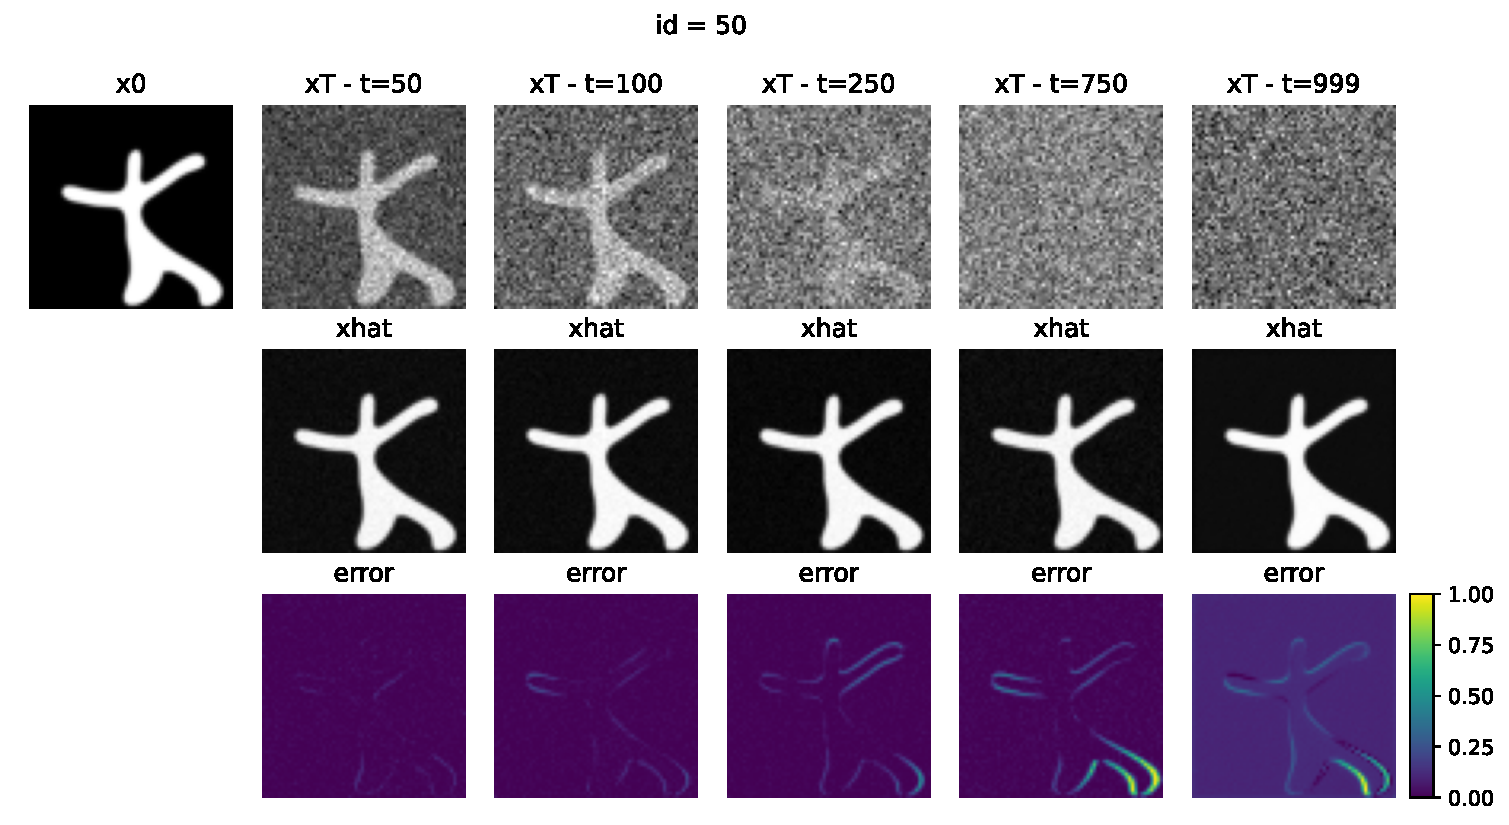
\includegraphics[width=0.75\linewidth]{figures/effect_noise_healthy.pdf}
    \caption{Effect of noise level on reconstructed images for healthy subject.}
    \label{fig:effect-noise-example-healthy}
\end{figure}

\begin{figure}[htbp]
  \centering
  \begin{subfigure}{0.75\linewidth}
    \includegraphics[width=\linewidth]{figures/effect_noise_darker_circle.pdf}
    \caption{Anomaly: \texttt{darker\_circle}}
  \end{subfigure}

  \begin{subfigure}{0.75\linewidth}
    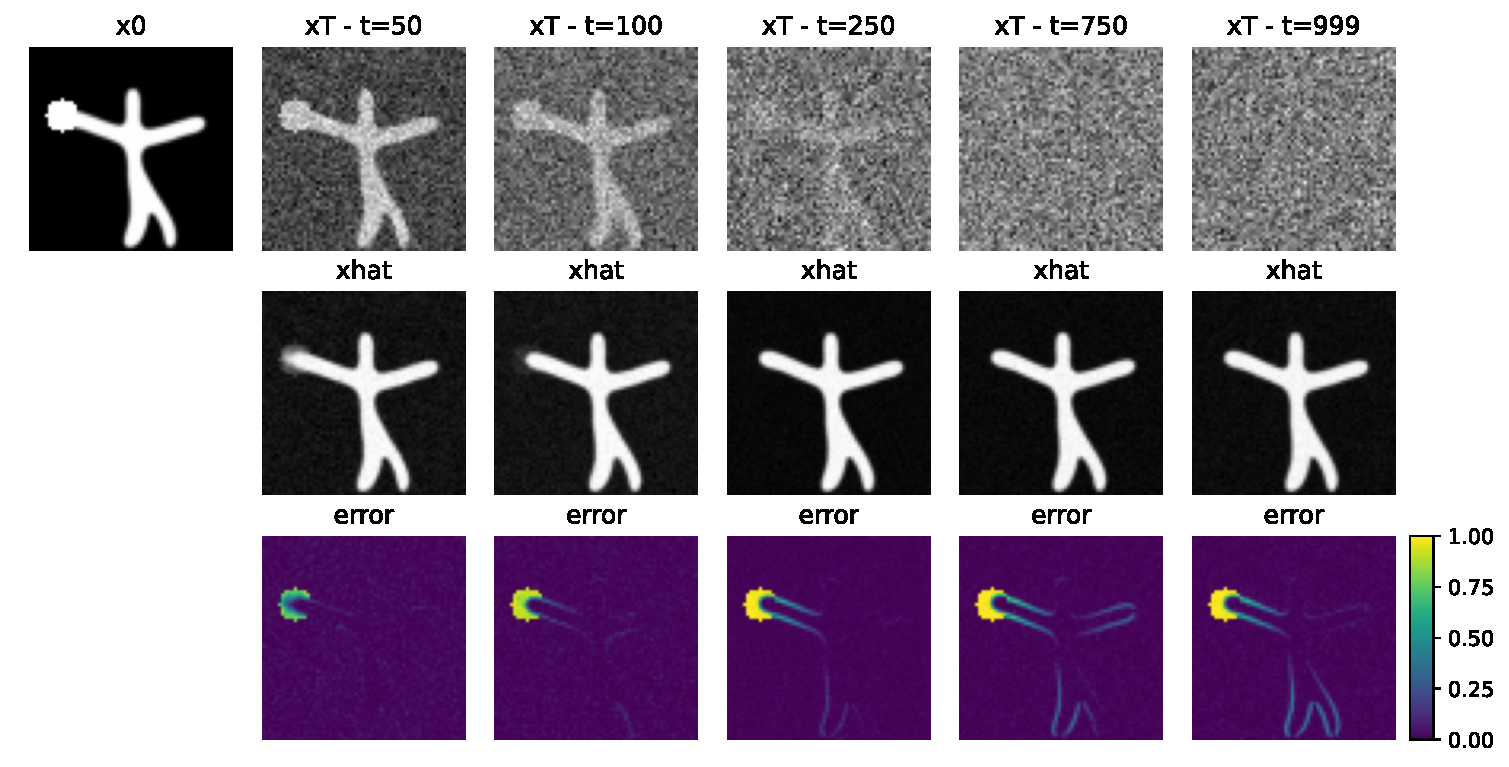
\includegraphics[width=\linewidth]{figures/effect_noise_growing_circle.pdf}
    \caption{Anomaly: \texttt{growing\_circle}}
  \end{subfigure}

  \caption{Effect of noise level on reconstructed images for anomalous subjects.}
  \label{fig:effect-noise-example-ano}
\end{figure}

\chapter{Feature Extractor Network}
\label{app:fe-layer}

\cref{fig:fe-layers} shows an example of feature maps from our feature extractor network $\text{FE} \Phi$. Each feature map is upscaled using linear interpolation to match the original spatial resolution of original image. The color displays the highest activation values across all channels at each pixel position, which is calculated as the mean of all channels. We observe that $\Phi$ effectively captures the perceptual structure of our figures at different scales. In particular, \texttt{stage2} focuses on overall shape of the \texttt{starman}, while \texttt{stage3} highlights the importance controlled points (head, legs and hands) of each figure. \texttt{stage4} operates at smallest resolution ($4, 4$), and due to the effect of upscaling, it does not capture any meaningful part of the original images that we can exploit. This is the reason why we utilize features from \{\texttt{stage2}, \texttt{stage3}\} to calculate our feature distances.

\begin{figure}[htbp]
  \centering
  \begin{subfigure}{0.75\linewidth}
    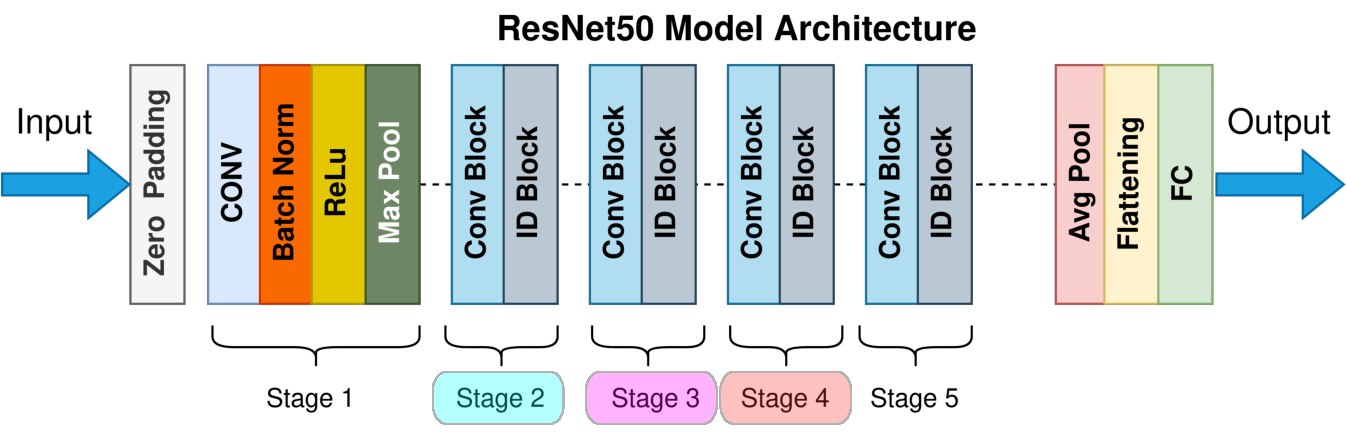
\includegraphics[width=\linewidth]{figures/resnet-50-arch.pdf}
    \caption{ResNet-50 architecture}
    \label{fig:resnet50-arch}
  \end{subfigure}

  \begin{subfigure}{0.75\linewidth}
    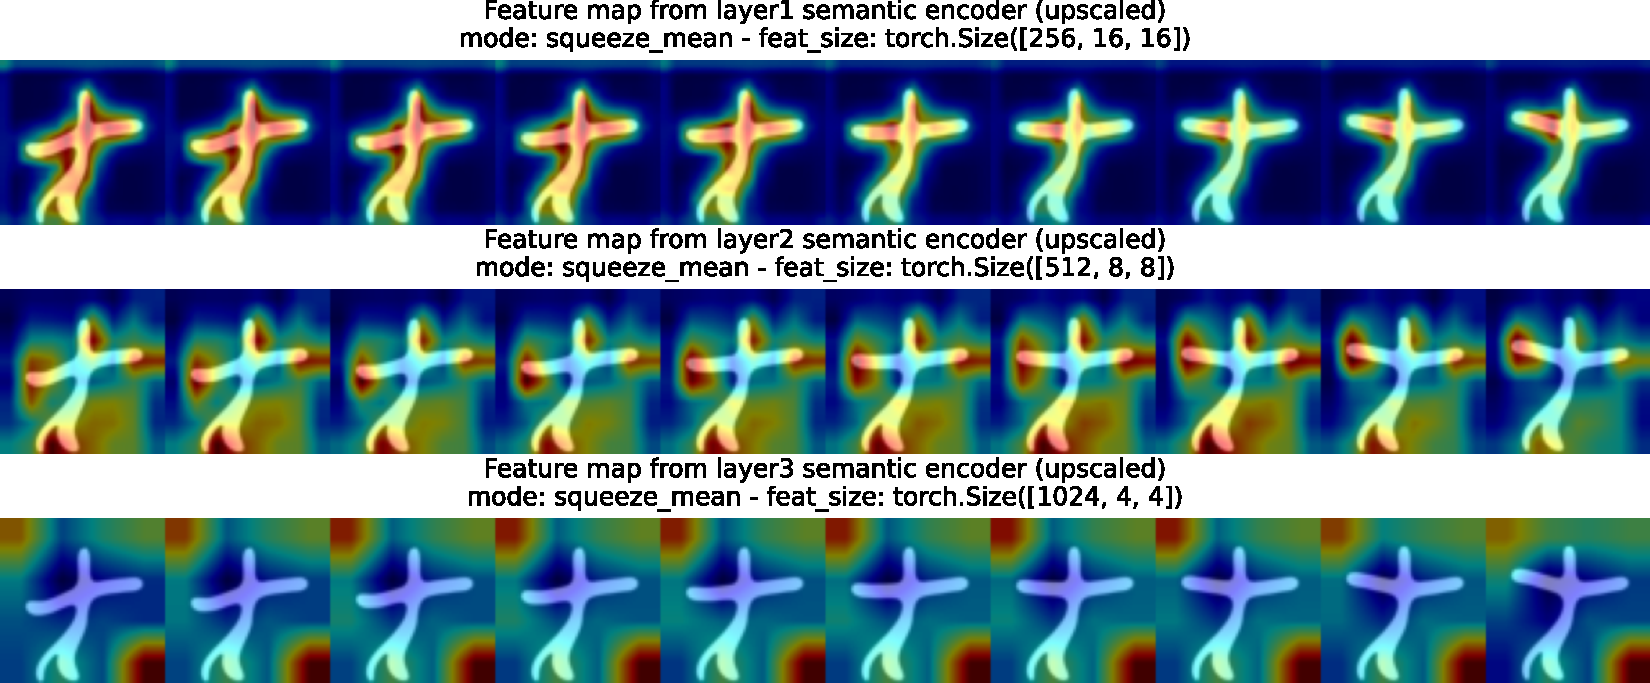
\includegraphics[width=\linewidth]{figures/fe-layer-healthy.pdf}
    \caption{Healthy subject}
    \label{fig:fe-layer-healthy}
  \end{subfigure}

  \begin{subfigure}{0.75\linewidth}
    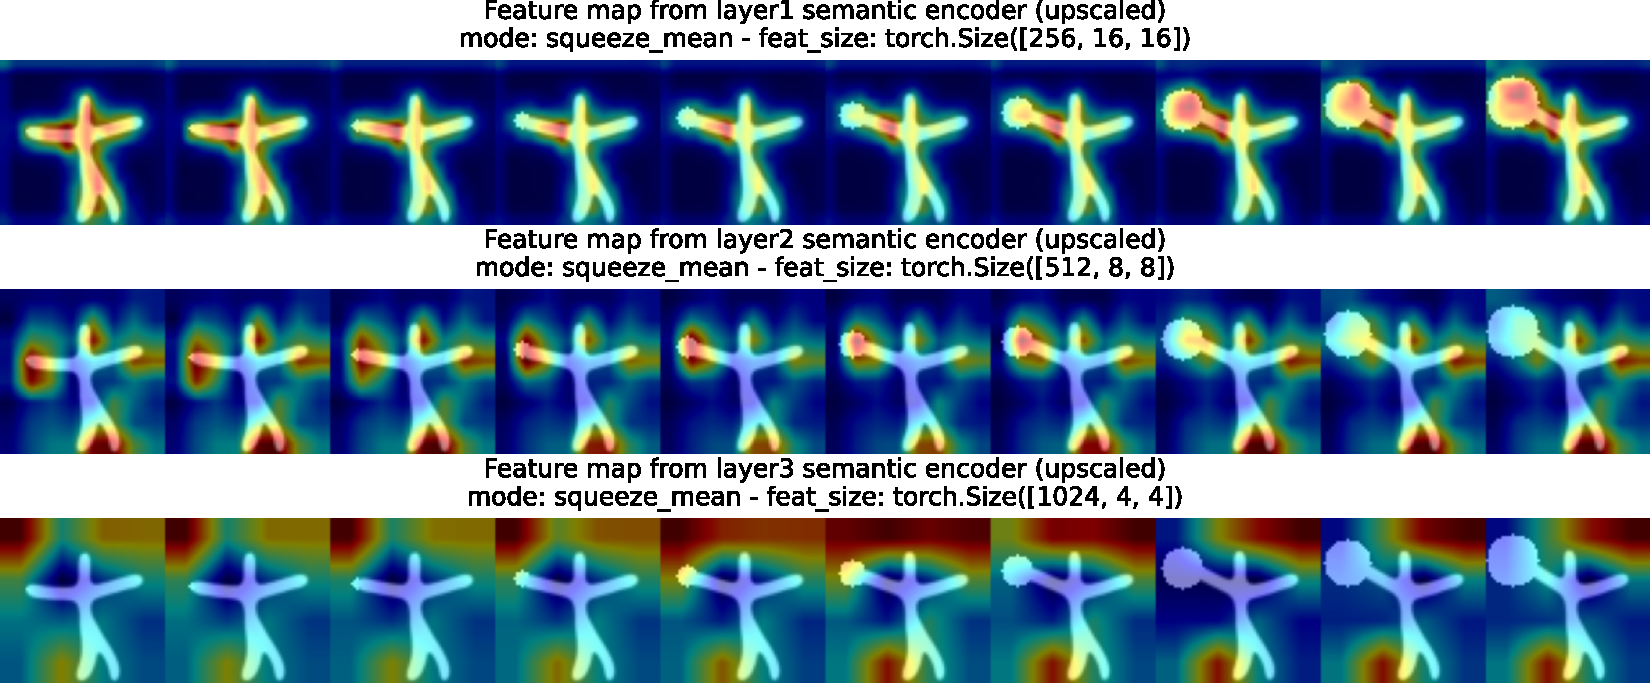
\includegraphics[width=\linewidth]{figures/fe-layer-anomaly.pdf}
    \caption{Anomaly subject}
    \label{fig:fe-layer-anomaly}
  \end{subfigure}
  \caption[Example feature maps from semantic encoder]{Example outputs from layers of Feature Extractor network $\Phi$ in \ac{SDM}. \cref{fig:resnet50-arch} shows ResNet-50 architecture. \cref{fig:fe-layer-healthy} and \cref{fig:fe-layer-anomaly} display example of outputs for healthy and anomalous subject, respectively. Notation: \texttt{stage2}, \texttt{stage3} and \texttt{stage4} from ResNet architecture correspond to \texttt{layer1}, \texttt{layer2} and \texttt{layer3} in our paper, respectively.}
  \label{fig:fe-layers}
\end{figure}

\chapter{Stochastic subcode manipulation}

We know that the stochastic subcode $\rvx_T^{\text{infer}}$ contains the fine-grained details about origin input, that the semantic encoder fails to capture. As shown in \cite{lozuponeLDAE2025,DiffAE}, this stochastic subcode, in combination with the semantic subcode from semantic encoder, is a powerful tool (latent variable) for us to manipulate the reconstructed images because they provide the best information of input. In this section, we show an example of utilizing this subcode to impute the missing images by interpolation. Given a starting time point $\mathbf{x}_{s}$ and ending time point $\mathbf{x}_{e}$, we can impute the missing images $\mathbf{x}_l$ at time point $s < l < e$ by interpolating both semantic subcode and stochastic subcode. From the two input time points, we can extract their semantic and stochastic representation $(\mathbf{y}_{\text{sem}}^s, \mathbf{y}_{\text{sem}}^e)$ and $(\mathbf{x}_{\text{infer}}^s, \mathbf{x}_{\text{infer}}^e)$, respectively. Based on these spaces, the intermediate semantic and stochastic subcode of $\mathbf{x}_l$ can be formulated using two methods, following \cite{lozuponeLDAE2025}:

\paragraph{\texttt{lerp-slerp} interpolation}: we perform linear interpolation in semantic space and spherical interpolation in stochastic one:

\begin{align*}
  \mathrm{LERP}(\mathbf{y}_{\text{sem}}^s, \mathbf{y}_{\text{sem}}^e; \alpha) &= (1 - \alpha) \mathbf{y}_{\text{sem}}^s + \alpha \mathbf{y}_{\text{sem}}^e \\
  \mathrm{SLERP}(\mathbf{x}_{\text{infer}}^s, \mathbf{x}_{\text{infer}}^e; \alpha) &=
  \frac{\sin((1 - \alpha)\theta)}{\sin(\theta)} \mathbf{x}_{\text{infer}}^s +
  \frac{\sin(\alpha \theta)}{\sin(\theta)} \mathbf{x}_{\text{infer}}^e
\end{align*}

where the angle $\theta$ between $\langle \mathbf{x}_{\text{infer}}^s, \mathbf{x}_{\text{infer}}^e \rangle$ is calculated as: 
\begin{align*}
    \theta = \arccos \left( \frac{\langle \mathbf{x}_{\text{infer}}^s, \mathbf{x}_{\text{infer}}^e \rangle}{\| \mathbf{x}_{\text{infer}}^s \| \cdot \| \mathbf{x}_{\text{infer}}^e \|} \right)
\end{align*}

Coefficient $\alpha$ is the offset of target time point $l$ with respect to the starting and ending time points, and is defined as $\alpha = \frac{l - s}{e - s}$. We note that $\alpha \in [0, 1]$. Subsequently, $\mathbf{x}_l$ is imputed as reconstruction (decode) image by using $(\mathbf{y}_{\text{sem}}^l, \mathbf{x}_{\text{infer}}^l)$

\paragraph{\texttt{lerp-lerp} interpolation}: we perform linear interpolation in both semantic and stochastic space, using the same above formulas. 

\cref{fig:interpolation-healthy} and \cref{fig:interpolation-ano} show quantitative examples of interpolation using both methods, for both healthy and anomalous subjects. 

\begin{figure}[htbp]
  \centering
  \begin{subfigure}{0.8\linewidth}
    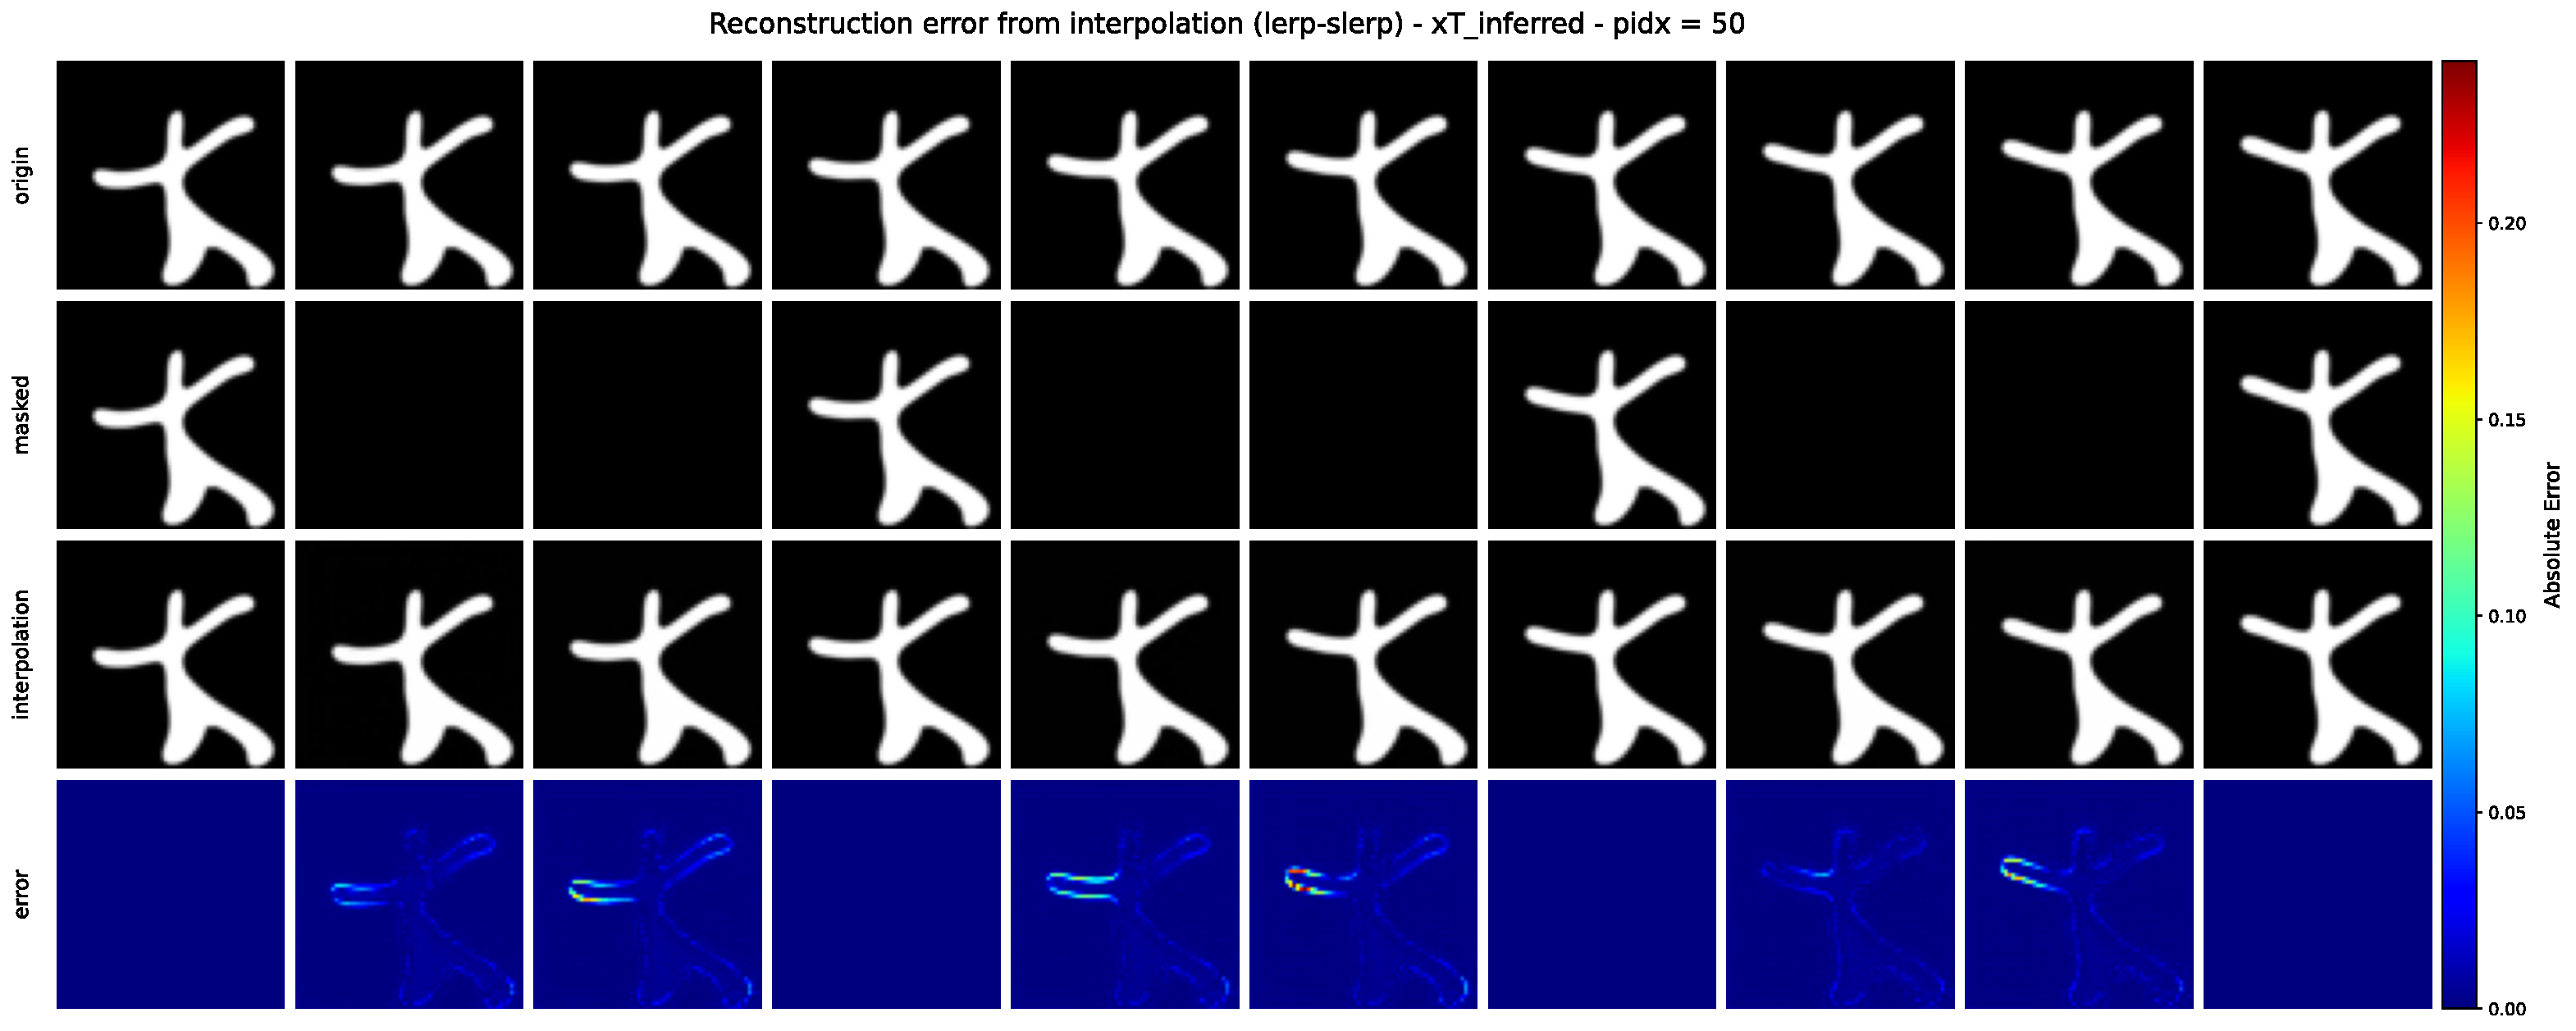
\includegraphics[width=\linewidth]{figures/interpolation-lerp-lerp-id-50.pdf}
    \caption{\texttt{lerp-lerp} interpolation}
  \end{subfigure}

  \begin{subfigure}{0.8\linewidth}
    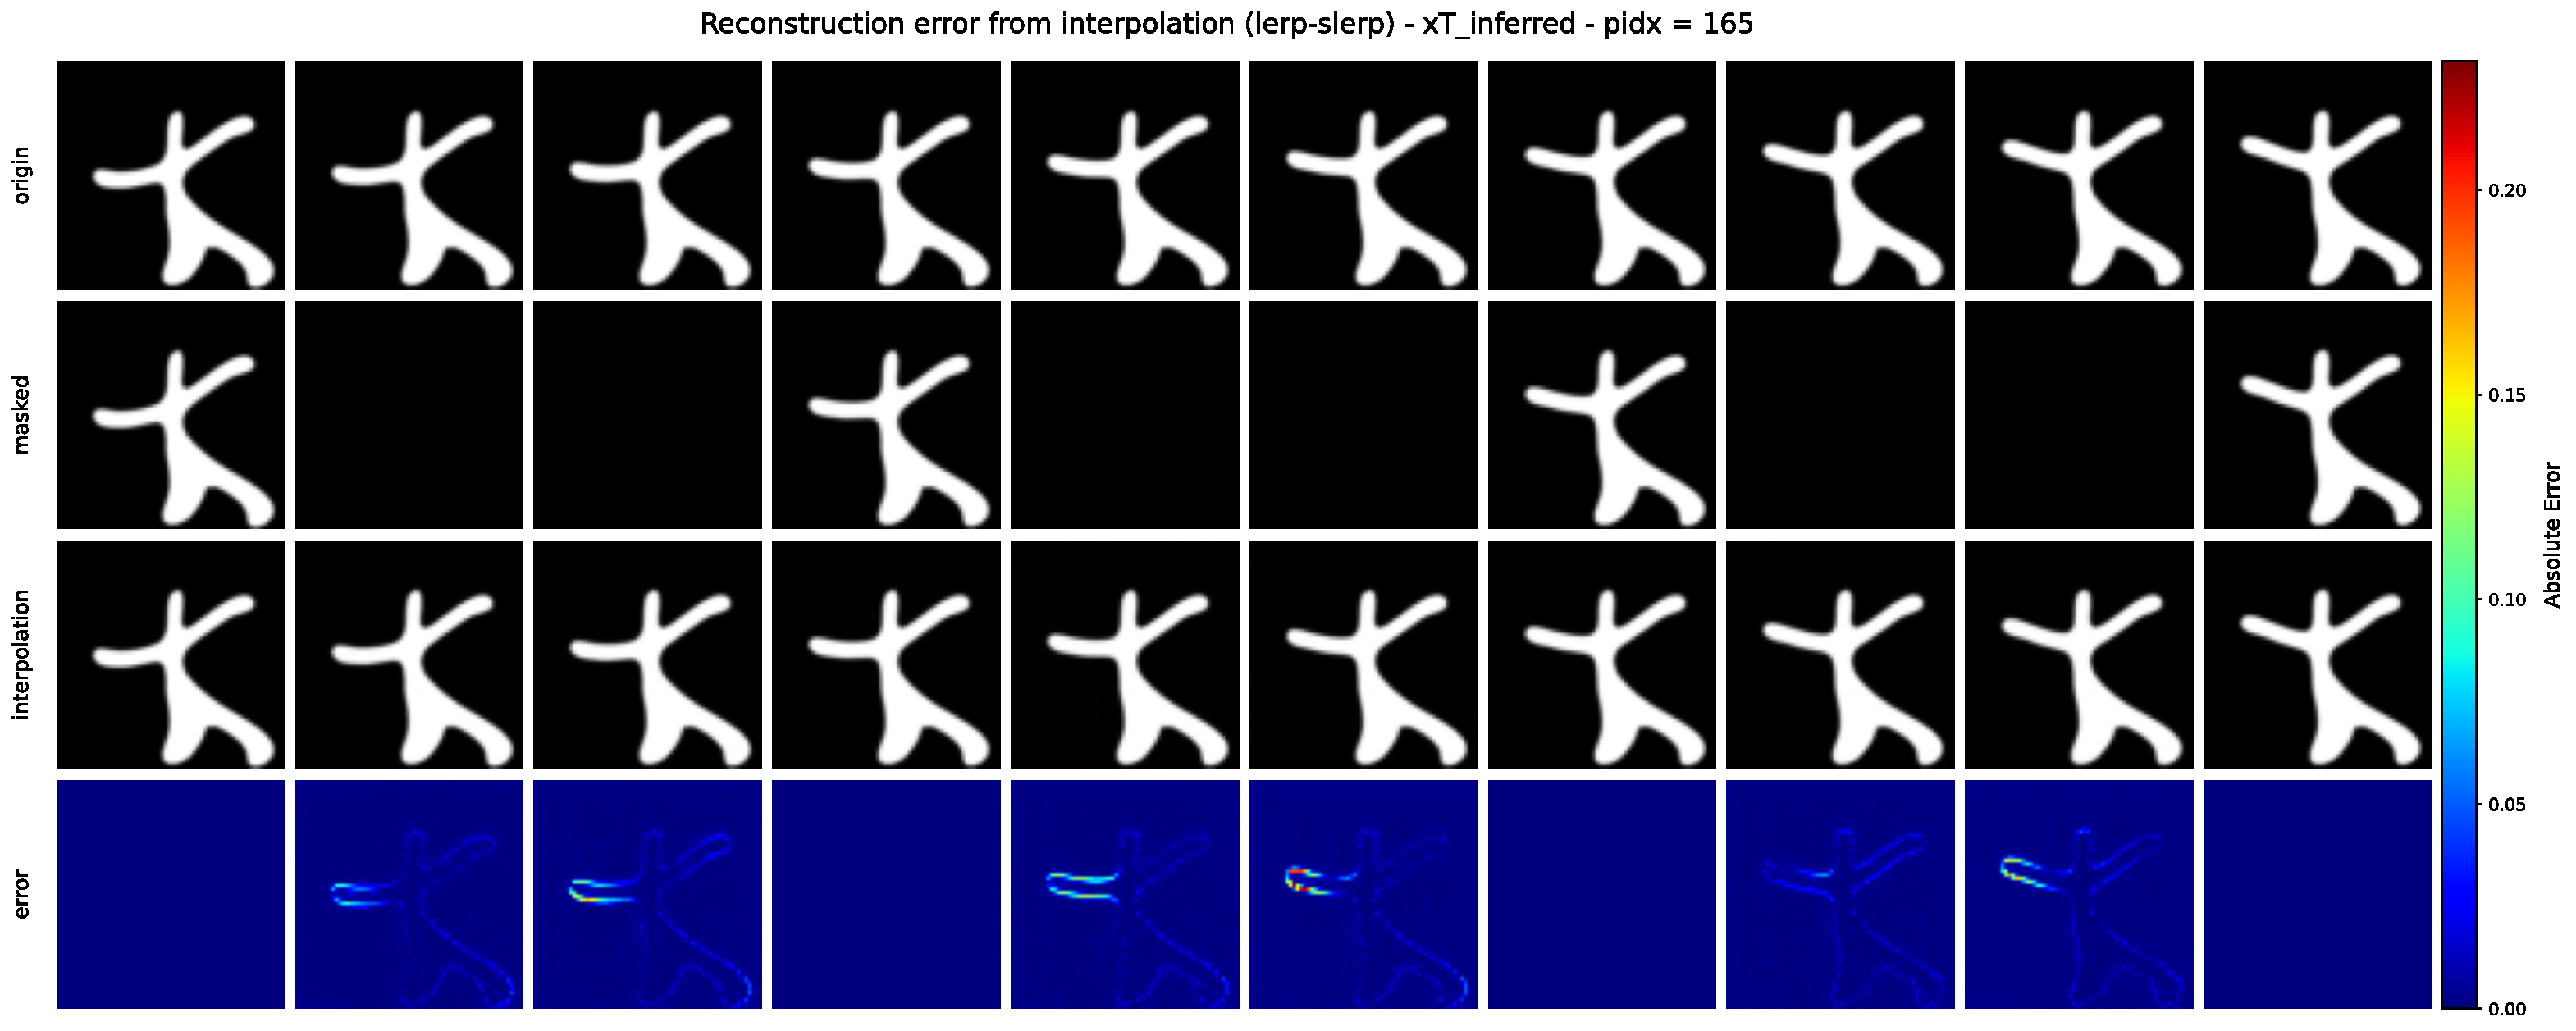
\includegraphics[width=\linewidth]{figures/interpolation-lerp-slerp-id-50.pdf}
    \caption{\texttt{lerp-slerp} interpolation}
  \end{subfigure}
  \caption{Interpolation from stochastic subcode for healthy subject. }
  \label{fig:interpolation-healthy}
\end{figure}

\begin{figure}[htbp]
  \centering
  \begin{subfigure}{0.8\linewidth}
    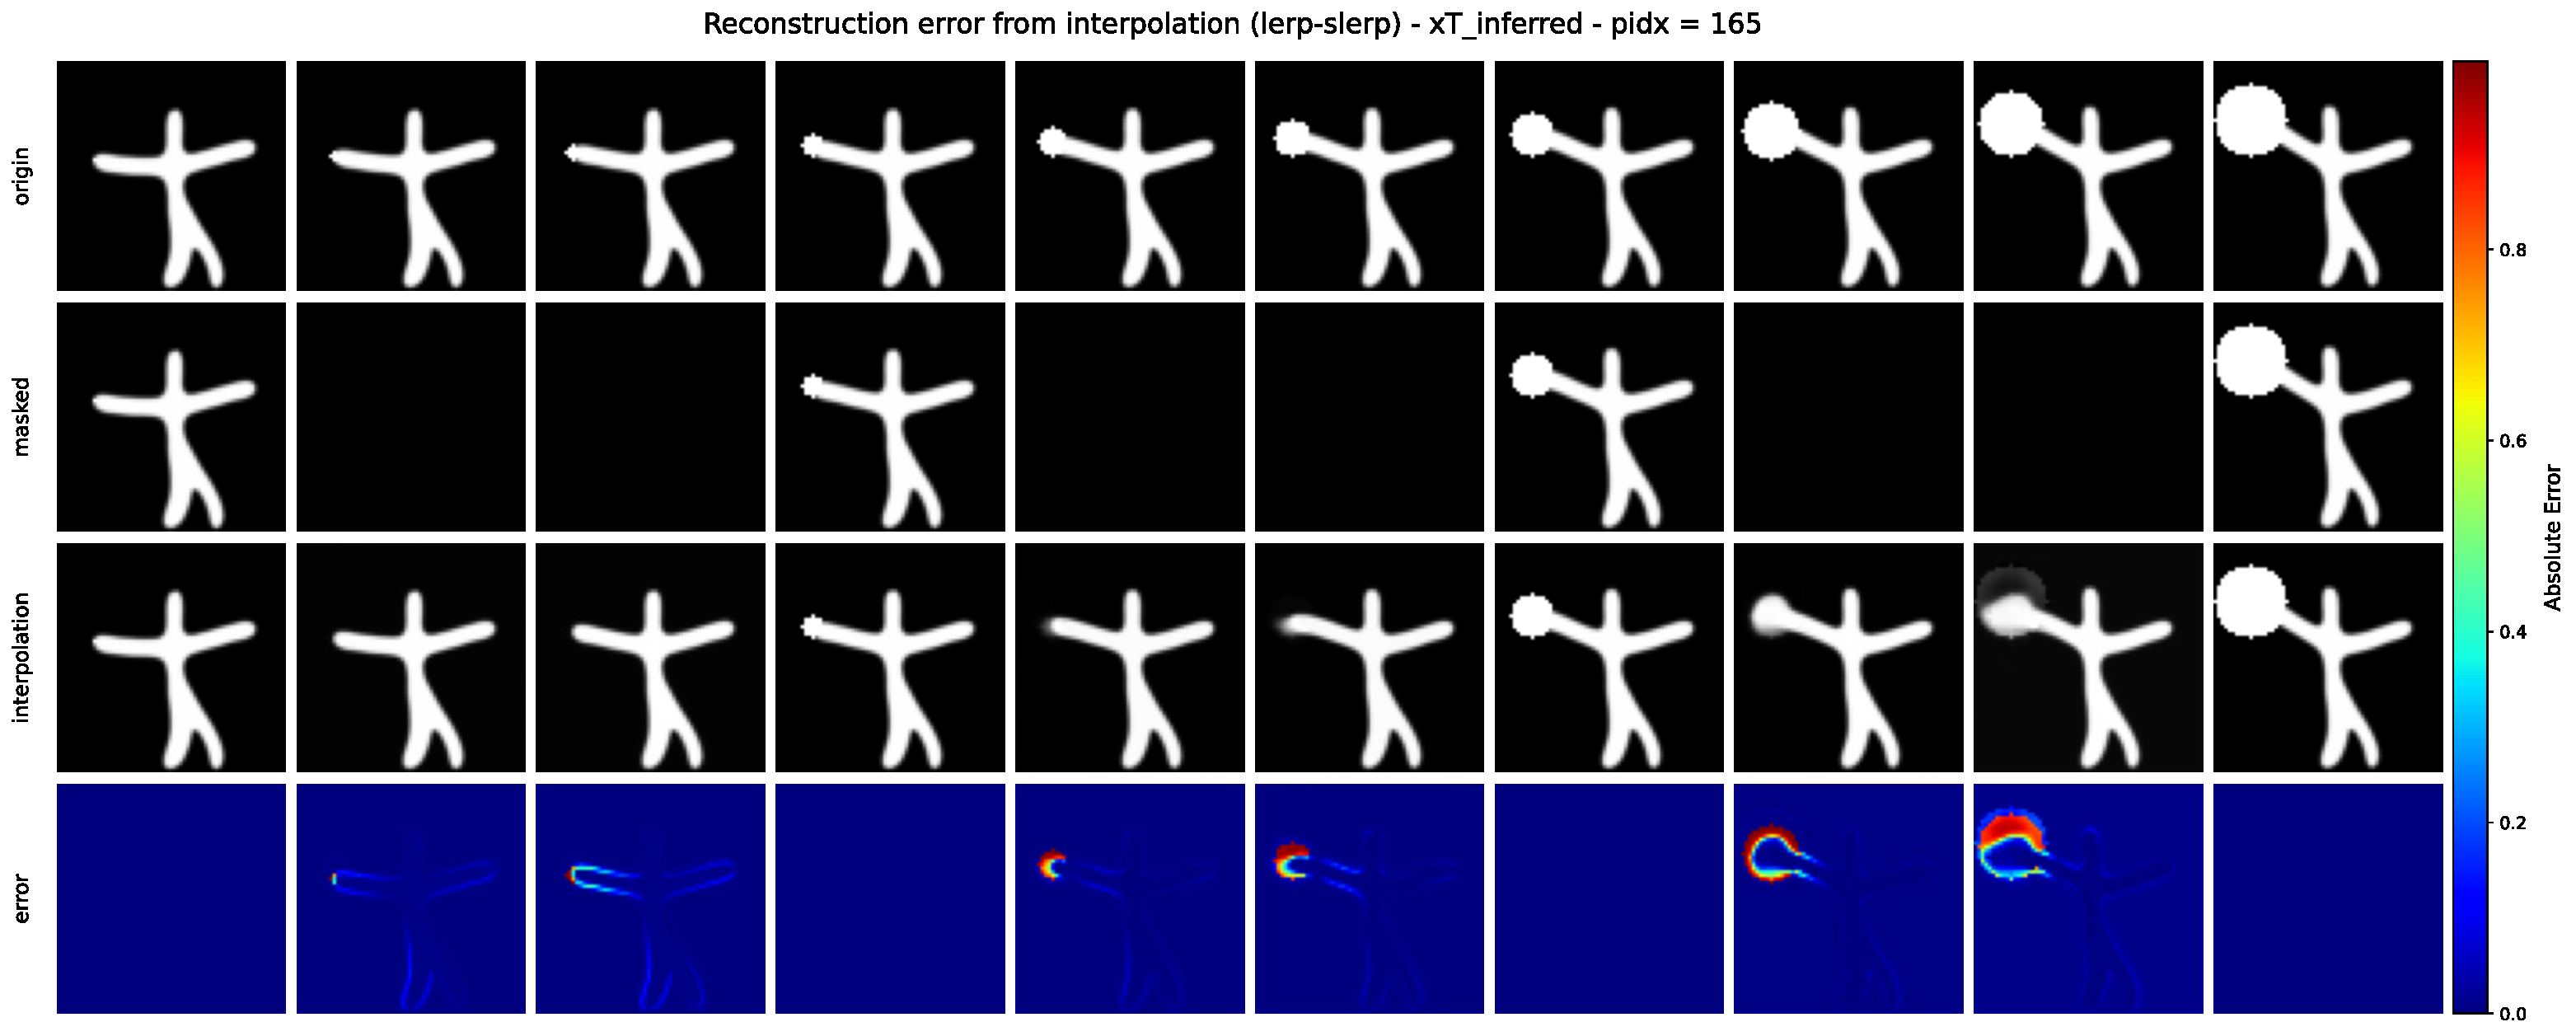
\includegraphics[width=\linewidth]{figures/interpolation-lerp-lerp-id-165.pdf}
    \caption{\texttt{lerp-lerp} interpolation}
  \end{subfigure}

  \begin{subfigure}{0.8\linewidth}
    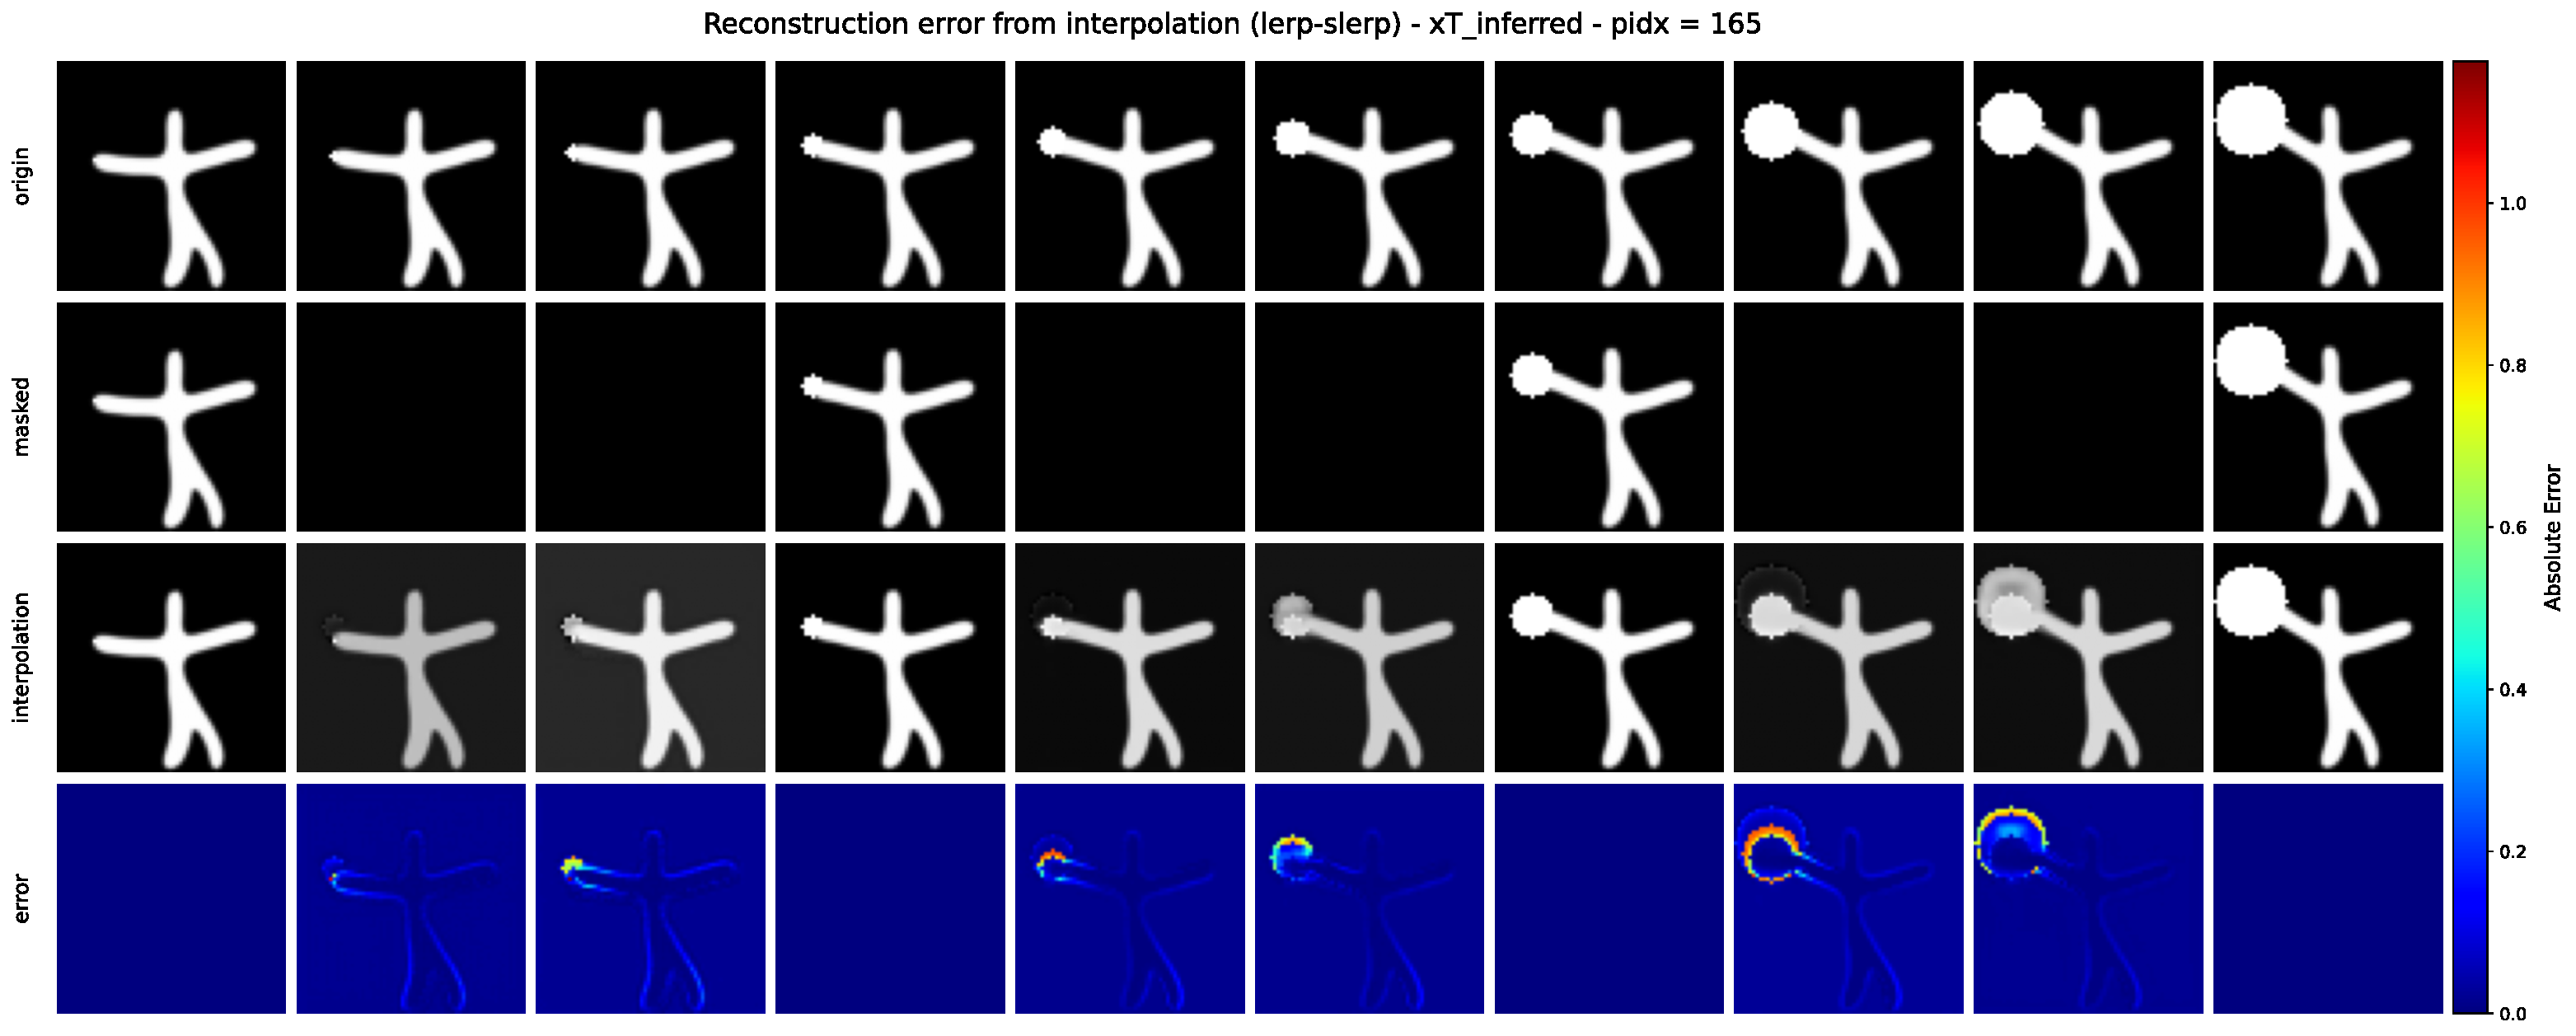
\includegraphics[width=\linewidth]{figures/interpolation-lerp-slerp-id-165.pdf}
    \caption{\texttt{lerp-slerp} interpolation}
  \end{subfigure}
  \caption{Interpolation from stochastic subcode for healthy subject. }
  \label{fig:interpolation-ano}
\end{figure}

% \clearpage
\chapter{More examples of LAFM Anomaly score maps}
\begin{figure}[htbp]
  \centering
  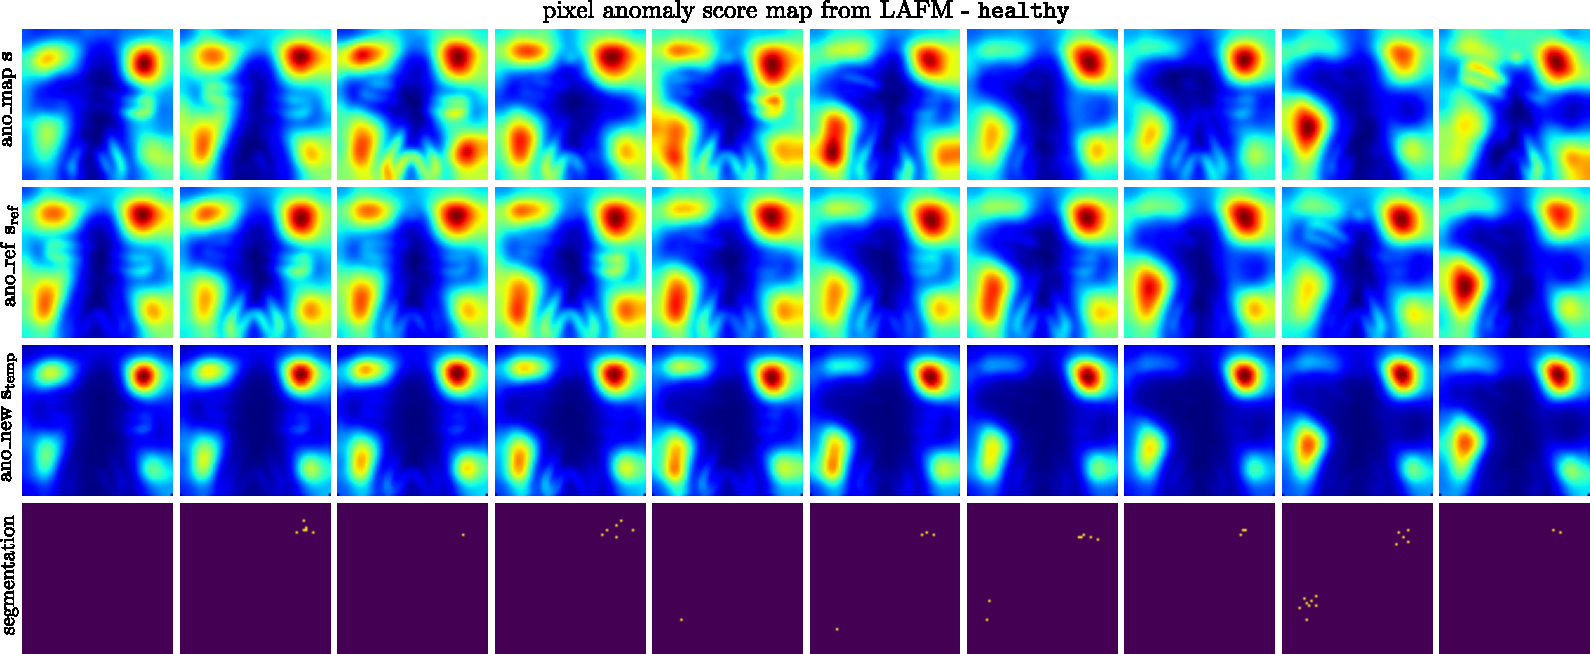
\includegraphics[width=0.75\linewidth]{figures/app-lafm-healthy.pdf}
  \caption[Example: anomaly segmentation from LAFM - \texttt{healthy} subject]{Example of anomaly score map from LAFM for healthy subject. From top to bottom: input score map (from FAM), anomaly map references, updated score map (LAFM), anomaly segmentation (Yen threshold).}
\end{figure}

\begin{figure}[htbp]
  \centering
  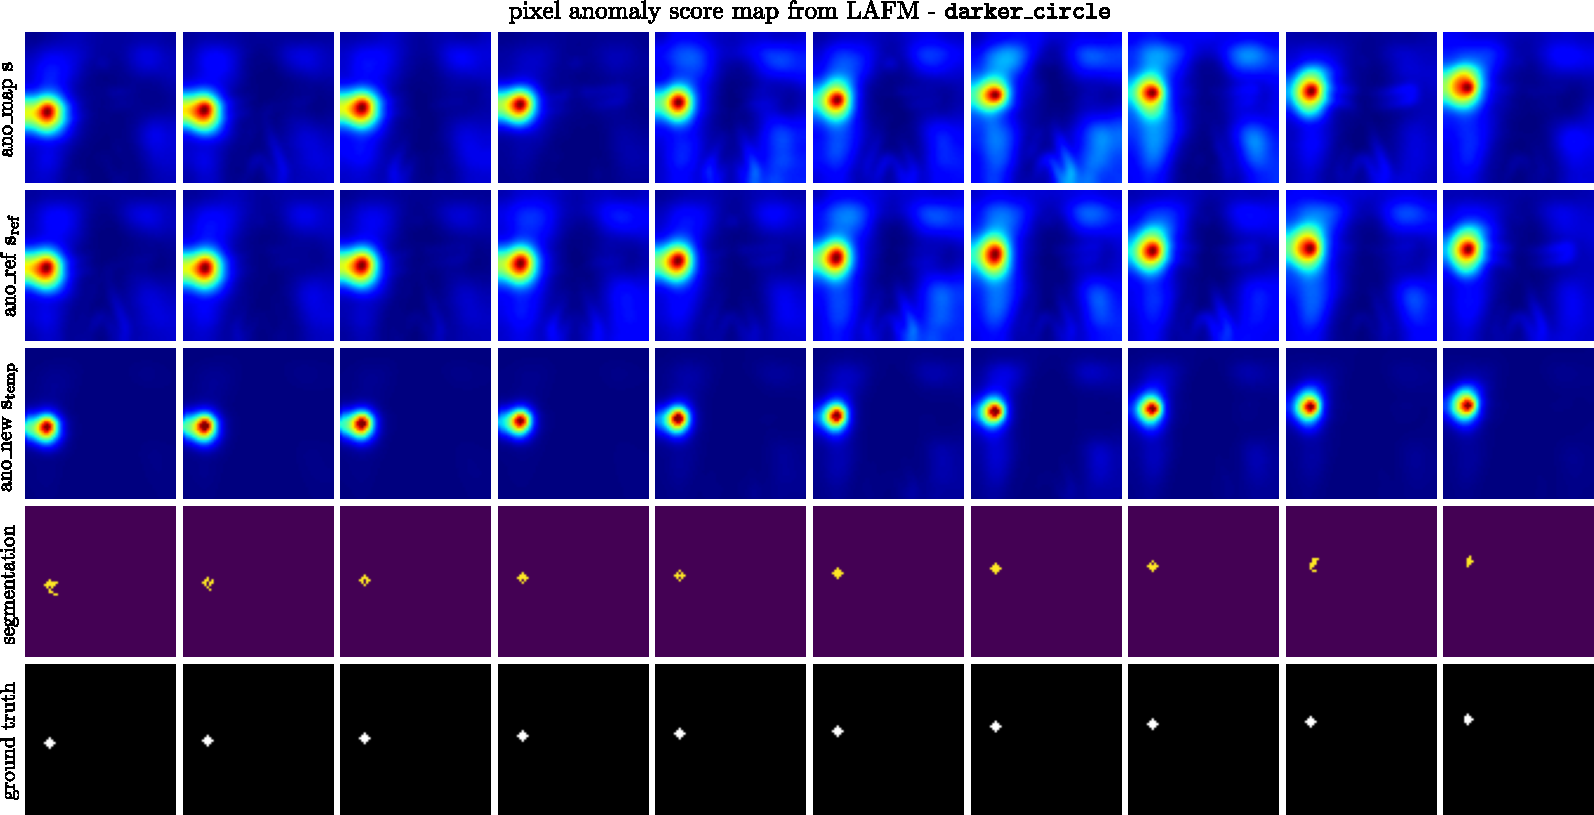
\includegraphics[width=0.75\linewidth]{figures/app-lafm-darkercircle.pdf}
  \caption[Example: anomaly segmentation from LAFM - \texttt{darker\_circle}]{Example of anomaly score map from LAFM for anomaly \texttt{darker\_circle} subject. From top to bottom: input score map (from FAM), anomaly map references, updated score map (LAFM), anomaly segmentation (Yen threshold) and ground truth annotation.}
\end{figure}

\begin{figure}[htbp]
  \centering
  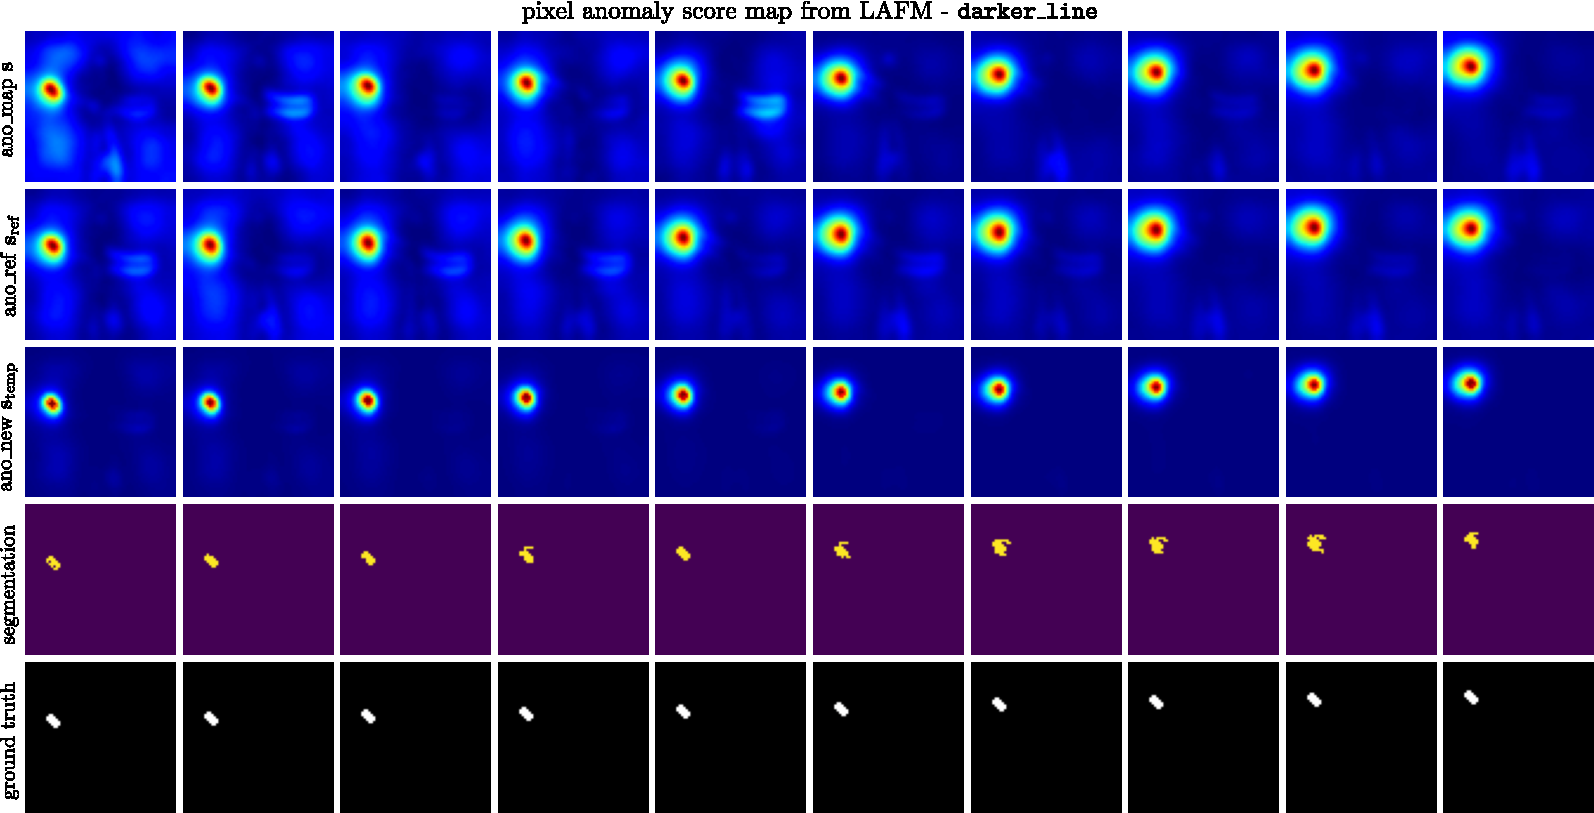
\includegraphics[width=0.75\linewidth]{figures/app-lafm-darkerline.pdf}
  \caption[Example: anomaly segmentation from LAFM - \texttt{darker\_line}]{Example of anomaly score map from LAFM for anomaly \texttt{darker\_line} subject. From top to bottom: input score map (from FAM), anomaly map references, updated score map (LAFM), anomaly segmentation (Yen threshold) and ground truth annotation.}
\end{figure}
\FloatBarrier


% References

\bibliographystyle{apalike}
\bibliography{anodiffbib}

\end{document}
